% =============================================================================
% ICLR 2026 submission draft.
% Paste this whole file into an Overleaf project that already contains the
% official ICLR 2026 style files (iclr2027_conference.sty / .bst), e.g. start
% from Overleaf's "ICLR 2026" template gallery entry and replace main.tex with
% this file. If the official style-file name differs from what is assumed
% below, just rename the \usepackage line accordingly -- nothing else in this
% document depends on the exact file name.
% =============================================================================
\documentclass{article} % For LaTeX2e
\usepackage{iclr2027_conference,times}

% ---- standard extra packages ----
\usepackage{graphicx}
\usepackage{booktabs}
\usepackage{amsmath}
\usepackage{amssymb}
\usepackage{natbib}
\usepackage{hyperref}
\usepackage{url}
\usepackage{xcolor}
\usepackage{listings}
\usepackage{multirow}
\usepackage{subcaption}
\usepackage{tikz}
\usetikzlibrary{arrows.meta,positioning,calc,fit,backgrounds,shapes.symbols}
\usepackage{enumitem}

\captionsetup{skip=4pt}
\setlength{\textfloatsep}{8pt plus 2pt minus 2pt}
\setlength{\floatsep}{6pt plus 2pt minus 2pt}
\setlength{\intextsep}{6pt plus 2pt minus 2pt}
\setlist{itemsep=1pt,topsep=2pt,parsep=0pt}

\lstset{
  basicstyle=\ttfamily\footnotesize,
  breaklines=true,
  columns=fullflexible,
  frame=single,
}

% \iclrfinalcopy % uncomment for camera-ready

\title{Any2Ego: Egocentric Viewpoint Translation\\
Taking Textual Modality as Anchor}

% Double-blind review: no author information in the submission version.
\author{Anonymous authors \\ Paper under double-blind review}

\newcommand{\fixme}[1]{\textcolor{red}{[FIXME: #1]}}

\begin{document}

\maketitle

\begin{figure*}[!ht]
\centering
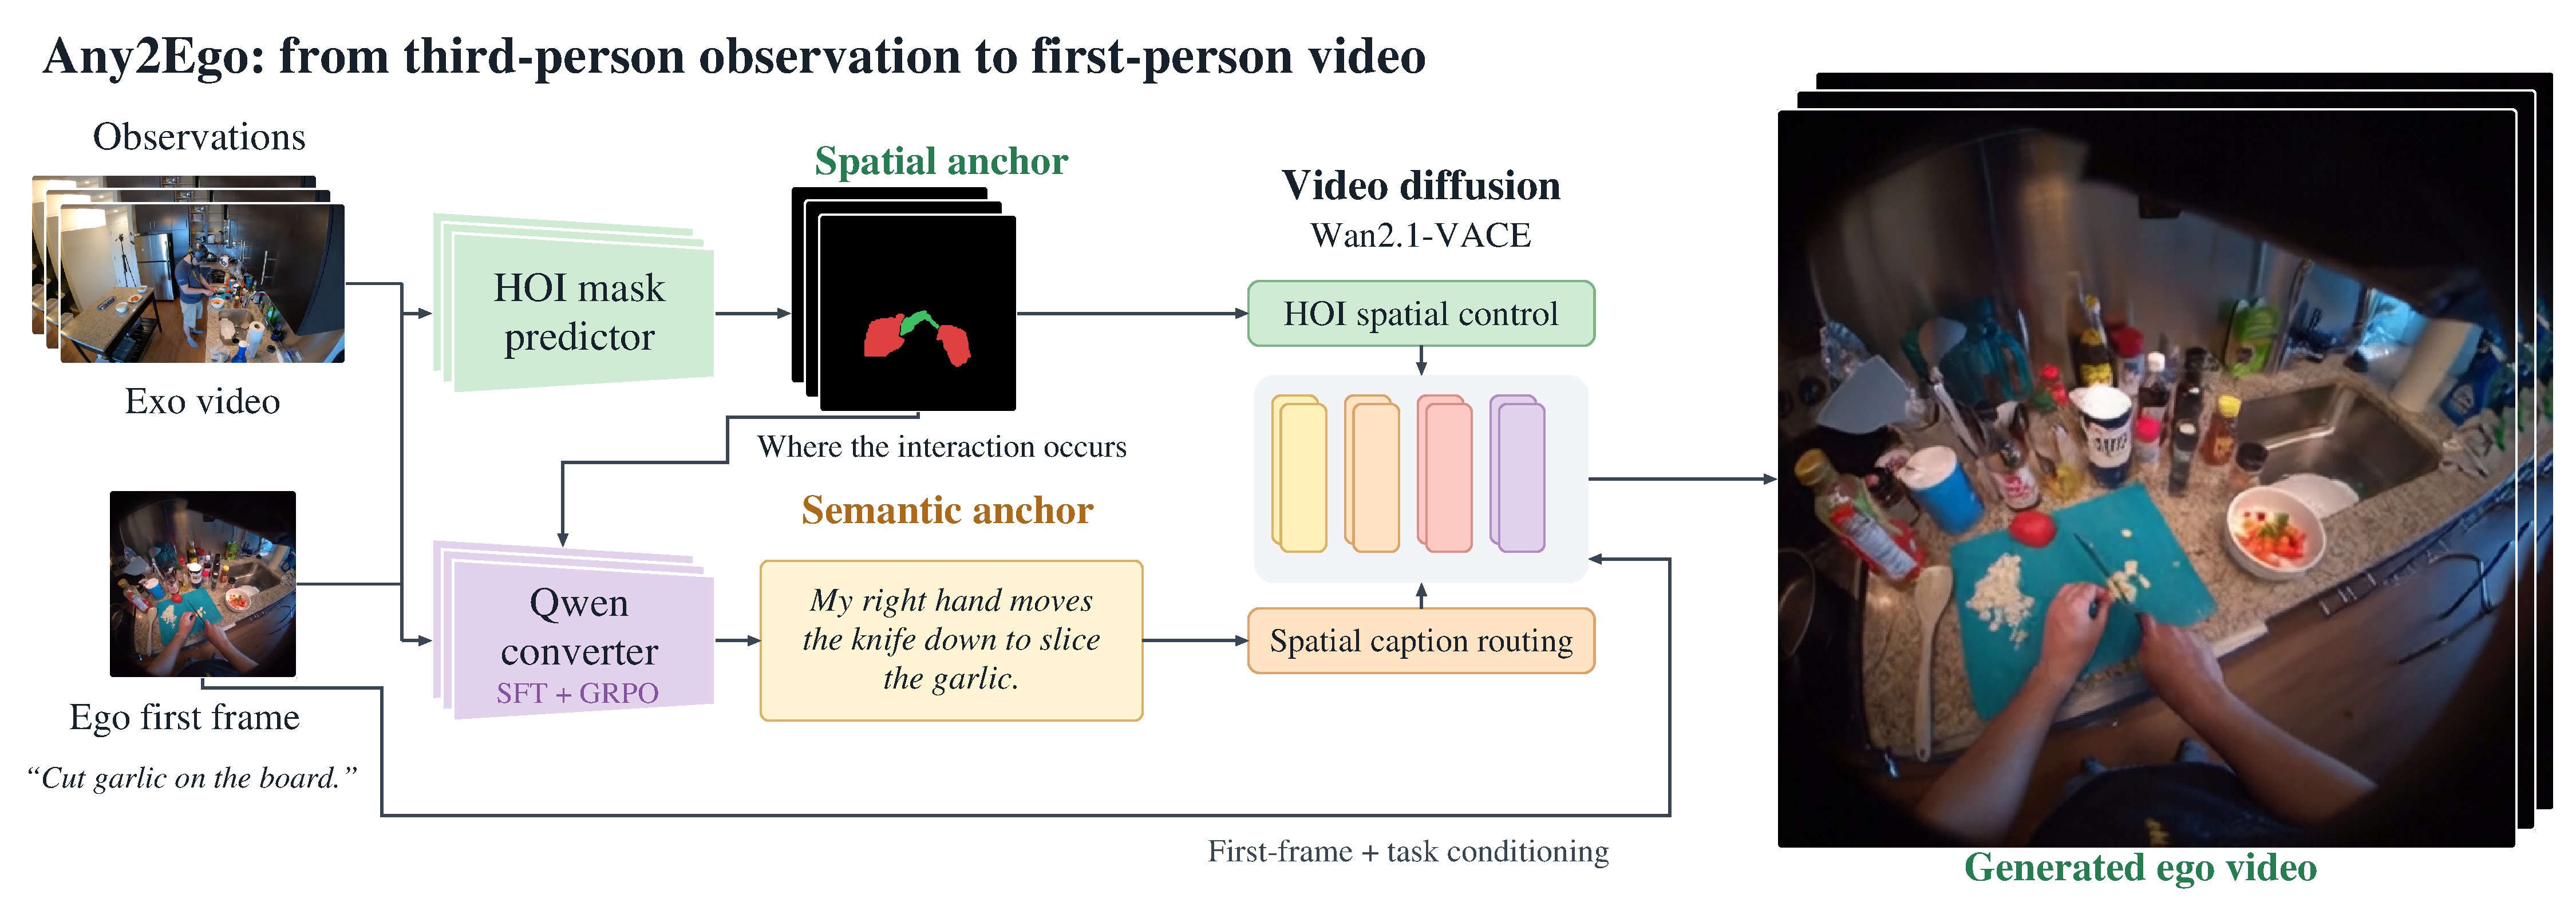
\includegraphics[width=\textwidth]{figs/teaser_overview.pdf}
\caption{\textbf{Any2Ego translates third-person observations into first-person videos.}
An HOI predictor provides the spatial anchor, while a Qwen converter trained
with SFT and GRPO supplies the first-person semantic anchor. HOI-conditioned
spatial routing controls where the caption enters video diffusion.
Input images, a generated caption excerpt, and the output video are integrated
into the schematic using one garlic-cutting example. The output stack shows
generated frames 1, 6, and 12, with frame 12 in front; colored mask symbols
schematically represent the spatial condition.}
\label{fig:any2ego_teaser}
\end{figure*}

\begin{abstract}
We present \textbf{Any2Ego}, a framework for egocentric viewpoint translation
-- synthesizing a first-person (ego) video of a manipulation task from a
third-person (exo) observation -- that replaces direct pixel-space mapping with
translation \emph{anchored on an explicit intermediate modality}. The
exo$\to$ego gap is too large to bridge end-to-end: the same action looks
entirely different across views, yet what is invariant is the interaction
itself -- which hand acts on which object, and where. We factor this invariant
into two complementary anchors: a \emph{spatial anchor} (a hand--object
interaction (HOI) mask, following prior work) that specifies \emph{where} the
interaction occurs, and -- our contribution -- a \emph{textual anchor}, a
natural-language ego-perspective caption
(``I see my hands holding a knife over an onion\dots'') that specifies
\emph{what} is happening. We train the producers of both anchors: a
Qwen3-VL-8B exo$\to$ego caption converter, via two-stage \textbf{SFT then
GRPO} training, that produces this caption \emph{deployably} -- from the exo
video, the ego first frame, and the HOI mask alone, never the ground-truth
ego frames, so the numbers below reflect the end-to-end pipeline, not an
oracle upper bound -- and, to remove the spatial anchor's oracle-mask
dependency at inference, a learned cross-view HOI-mask predictor
($\Phi_{\text{seg}}$). Feeding this deployable caption into a
mask-conditioned video-diffusion backbone (Wan2.1-VACE), we show that
\emph{how} it is injected is decisive, comparing three designs: (i)
mask-only, no caption (\textbf{base}); (ii) a naive \textbf{global} scalar
gate on an auxiliary caption cross-attention branch; and (iii) a per-token
\textbf{spatial-routing} gate that reuses the mask's own dense HOI features
to localize where the caption is applied. We evaluate on a fixed
$N{=}1{,}000$ EgoExo4D test pool against the real future ego frames, and we
report \textbf{FVD as the primary metric} for a measured reason: on a
$\sim\!1.6$\,s horizon an ego clip is largely static, so frame-level
fidelity pays out heavily for merely holding the given first frame -- a
no-model control that repeats that frame $13$ times attains $0.601$ SSIM at
$21.88$\,dB and thereby exceeds \emph{every} published baseline we evaluate
on all three frame-level metrics. We put the same control through FVD and it
scores $357.2$, worse than every generative baseline except two degenerate
ones and $10.7\times$ worse than our best arm: the freeze that tops the
frame-level table sits near the bottom of the distributional one. On FVD, the ordering
base $\to$ global gate $\to$ spatial route is
$42.6\!\to\!37.8\!\to\!33.3$, against $121.6$--$177.0$ for image-to-video
baselines and $1118.7$/$2361.1$ for exo-conditioned video-to-video
baselines: our weakest arm is $2.9\times$ better than the strongest
baseline. The frame-level metrics, read against that control, agree wherever
they can resolve a difference -- SSIM $0.608\!\to\!0.636\!\to\!0.660$, PSNR
$21.1\!\to\!21.7\!\to\!22.3$, LPIPS $0.194\!\to\!0.163\!\to\!0.144$ --
monotonic and uninverted, with spatial routing best and the global gate
second on every metric. A component ablation confirms both anchors are
load-bearing rather than decorative: at inference, randomizing only the
caption's content (mask held real) costs $3\%$ PSNR / $4\%$ SSIM / $15\%$
LPIPS relative to the full model (which still wins on $88.7\%$ of clips),
while randomizing only the mask's spatial content (caption held real) costs
$27\%$ PSNR / $36\%$ SSIM / $2.5\times$ LPIPS (full wins $100\%$) -- the mask
supplies the dominant spatial skeleton, the caption a smaller but consistent
semantic refinement. We position spatial-routing text injection, together
with its trained captioner, as a validated instantiation of the textual
anchor.

\end{abstract}

\section{Introduction}
\label{sec:intro}

Generating an egocentric (ego) video from an exocentric (exo) observation
requires preserving the observed action while translating the appearance
and layout of the scene into a first-person view.
Figure~\ref{fig:any2ego_teaser} illustrates this transformation with a
garlic-cutting example. The ego output must preserve the relation between
the hands, knife, and garlic while reconstructing the surrounding kitchen
from the wearer's viewpoint. Any2Ego makes these requirements explicit
through a spatial interaction anchor and a first-person semantic anchor,
then combines them through spatially routed video generation.

Prior work such as EgoExo-Gen \citep{xu2025egoexogen} conditions ego-video
generation on an exo video and the ego first frame, using hand--object
interaction (HOI) masks to transfer spatial structure across views. This
provides an explicit description of \emph{where} the hands and manipulated
objects are. However, a mask alone does not specify object appearance,
the meaning of a contact, or how the surrounding scene should be described
from the ego viewpoint. These missing semantics leave the generator with
ambiguities that spatial guidance alone cannot resolve.

We introduce \textbf{Any2Ego}, which complements the spatial HOI anchor
with a \emph{textual semantic anchor}. A Qwen-based cross-view converter
produces a structured ego-perspective caption from the exo video, ego first
frame, HOI mask, and task narration, describing the interaction and scene
in first-person terms. We train this converter with difference-weighted supervised
fine-tuning, followed by GRPO \citep{shao2024grpo} using a reward derived
from generated video previews. The two stages encourage captions to add
useful information beyond the existing conditions and to remain relevant
to downstream generation. A dedicated caption cross-attention branch
injects this semantic anchor alongside the spatial-control branch.

Providing the caption is only part of the solution: its influence should
also vary across the generated frame. A global scalar gate scales caption
features uniformly, even though different locations require different
semantic refinements. We therefore introduce an \emph{HOI-conditioned
spatial-routing module}. It reuses the spatial branch's dense features to
predict a gate for each video token and modulates the caption-attention
output accordingly. This lets the generator combine spatial constraints
with location-dependent semantic guidance, with the aim of reducing
structural distortions and preserving scene relationships across views.

\paragraph{Related work and remaining gap.}
\label{sec:related}
Existing approaches supply different parts of this solution.
EgoExo-Gen \citep{xu2025egoexogen} emphasizes cross-view HOI structure;
we adopt its mask-prediction formulation as our spatial component.
EgoX \citep{kang2025egox} instead constructs a geometric ego-view prior
through depth, point-cloud reconstruction, and camera poses. These spatial
representations motivate explicit intermediate conditions, but our focus is
on complementing them with ego-view semantics and controlling where those
semantics enter generation. General video models such as Stable Video
Diffusion \citep{blattmann2023svd}, ConsistI2V \citep{ren2024consisti2v},
and Wan \citep{wan2025} provide strong synthesis backbones, while VACE
\citep{vace2025} supports visual conditioning and editing. Their generic
conditioning interfaces do not by themselves provide the cross-view
semantic conversion and HOI-conditioned caption routing studied here.
Any2Ego connects these two operations within a spatially guided generator.

Our contributions are threefold:
\begin{itemize}
  \item A spatial--semantic intermediate representation for exo$\to$ego
  video generation, combining an HOI anchor with an ego-perspective
  textual anchor to describe both interaction geometry and scene semantics.
  \item A cross-view caption converter trained with difference-weighted
  SFT and generation-grounded GRPO, producing structured ego descriptions
  that serve as semantic conditions for the video generator.
  \item An HOI-conditioned, per-token routing module for caption
  cross-attention, evaluated against HOI-only and global-gate variants
  through generation comparisons, caption-quality evaluation, and
  component ablations.
\end{itemize}

\section{Method}
\label{sec:method}

\subsection{Framework overview}
\label{sec:overview}

We construct Any2Ego with a cross-view mask predictor $\Phi_{\mathrm{seg}}$,
a Qwen caption converter $\Phi_{\mathrm{cap}}$, and a video generator
$\Phi_{\mathrm{gen}}$ based on Wan2.1-VACE-1.3B \citep{wan2025,vace2025}.
Let $X=\{X_t\}_{t=0}^{T-1}$ denote the exo video, $S$ its HOI masks,
$I_0$ the ego first frame, $M_0$ its mask, and $n$ the task narration.
The predictor estimates the ego interaction geometry, the converter describes
it in first-person language, and the generator synthesizes the ego video:
\begin{equation}
\begin{aligned}
\widehat M &= \Phi_{\mathrm{seg}}(X,S,I_0,M_0),\\
c &\sim \Phi_{\mathrm{cap}}(\,\cdot\mid X,I_0,\widehat M,n),\qquad
\widehat Y = \Phi_{\mathrm{gen}}(I_0,\widehat M,n,c).
\end{aligned}
\label{eq:method-pipeline}
\end{equation}
The mask sequence $\widehat M$ and caption $c$ provide complementary spatial
and semantic conditions. We describe their construction first, then explain
how both conditions enter the generator in Section~\ref{sec:condition-injection}.

\begin{figure*}[t]
\centering
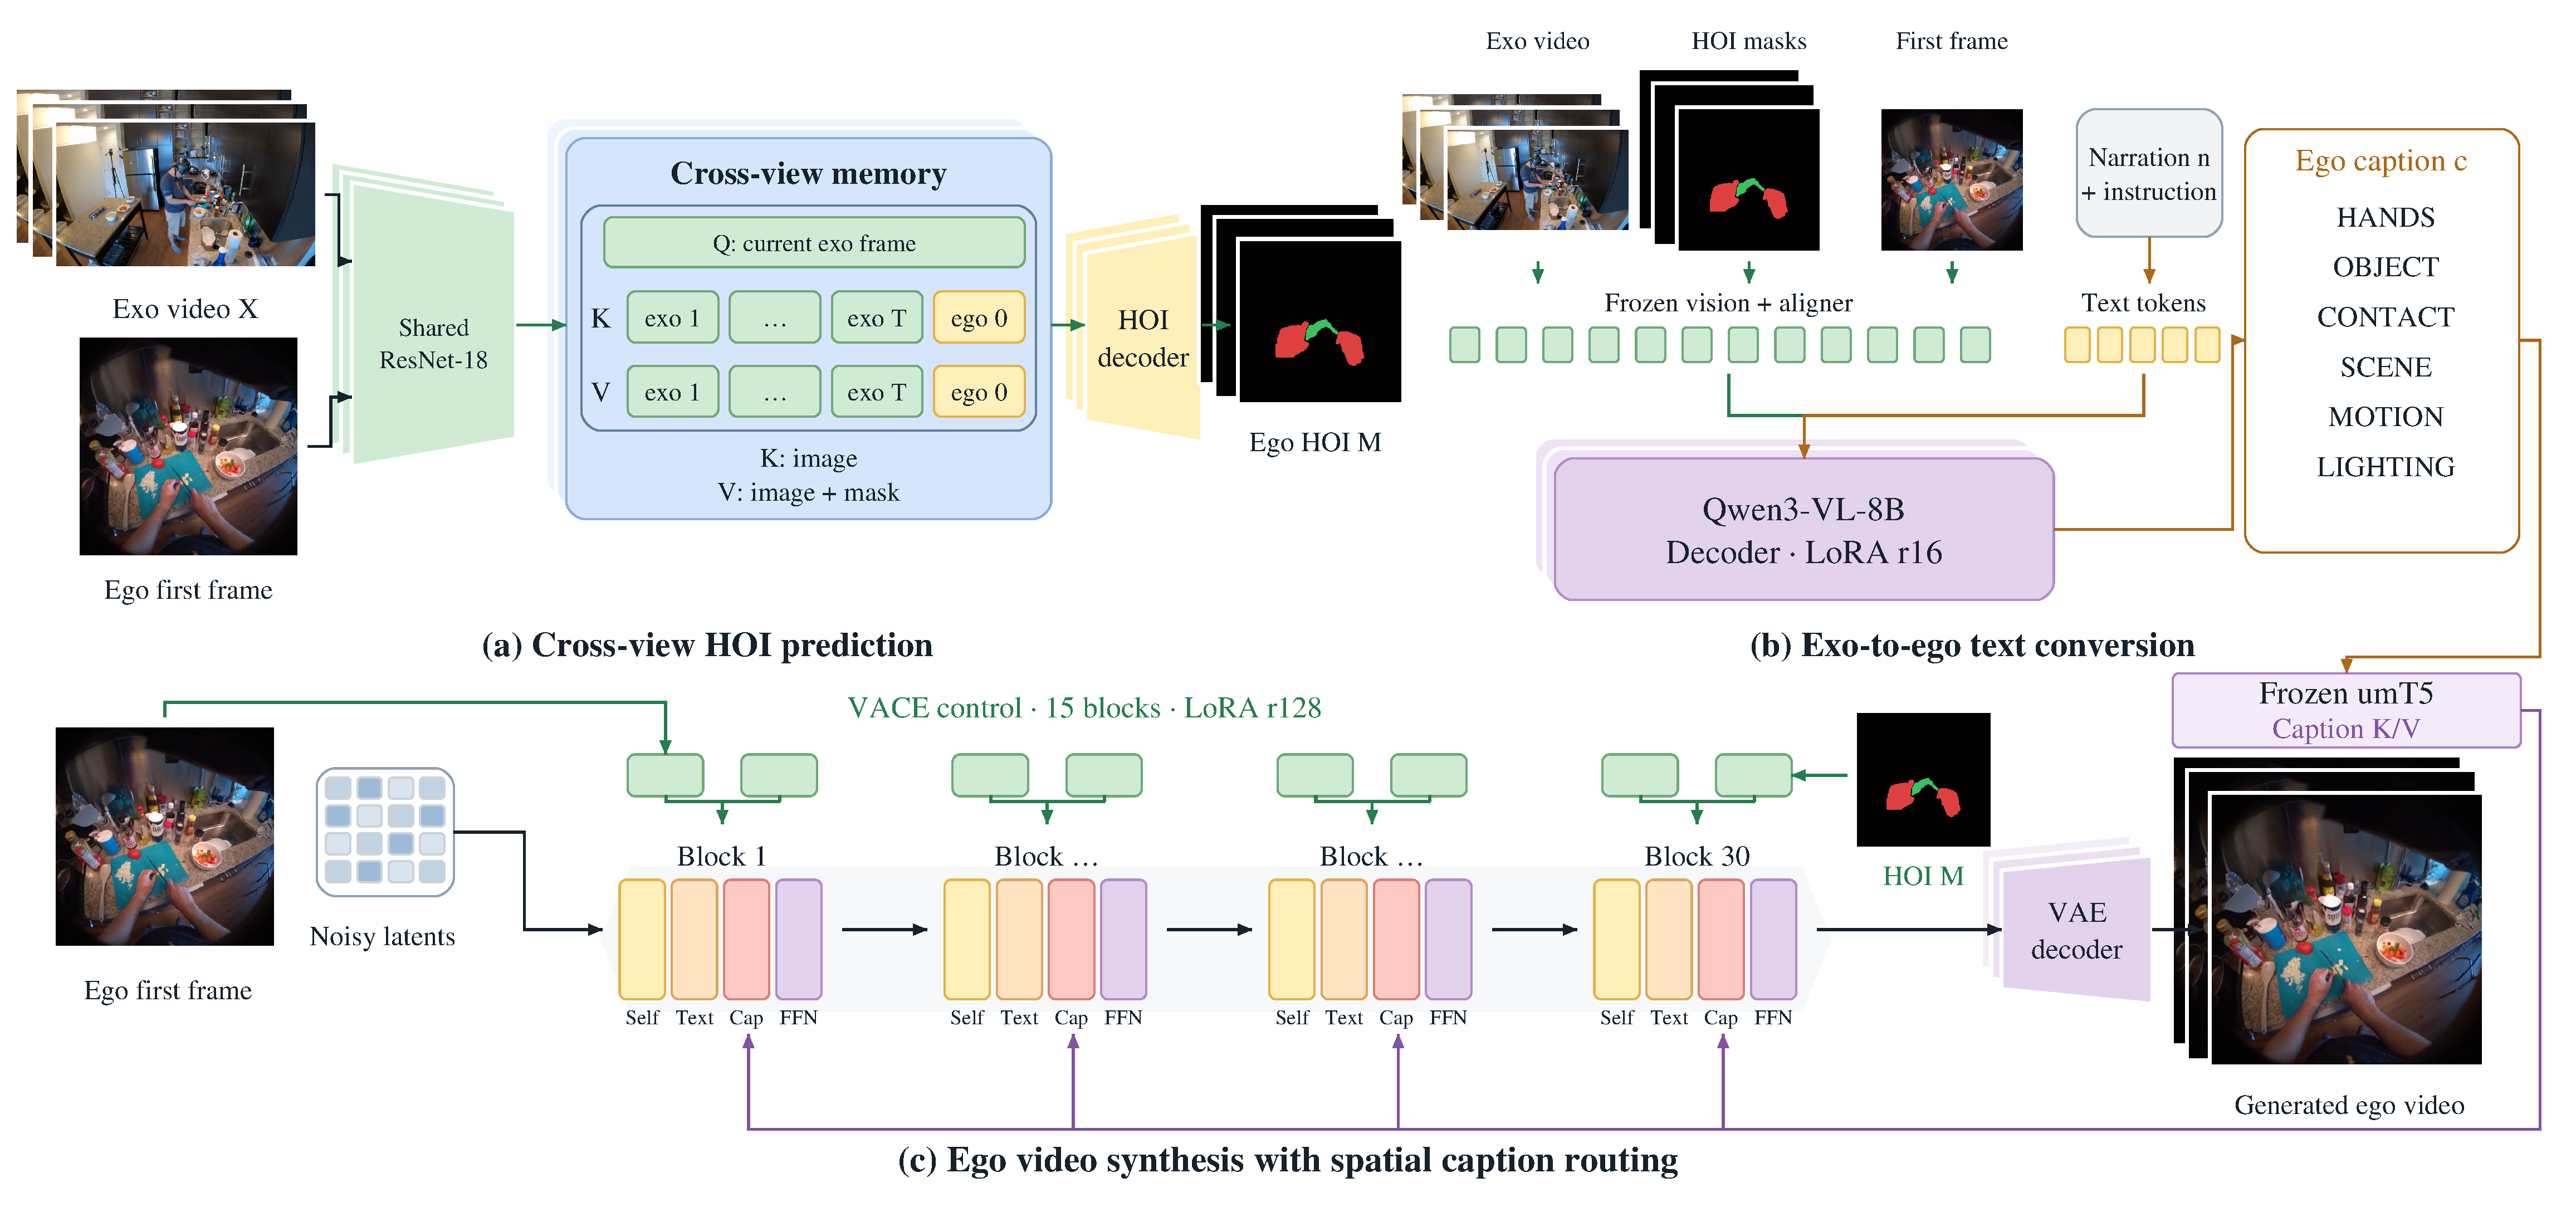
\includegraphics[width=\textwidth]{figs/architecture_illustration.pdf}
\caption{\textbf{Any2Ego pipeline.} The cross-view mask predictor estimates
an ego HOI-mask sequence; the Qwen converter generates a structured
first-person caption; and the video generator combines these spatial and
semantic conditions. Sections~\ref{sec:phiseg-method} and
\ref{sec:student-method} describe the converters; Section~\ref{sec:condition-injection}
describes condition injection and generator training.}
\label{fig:pipeline}
\end{figure*}

\subsection{Cross-view HOI-mask predictor}
\label{sec:phiseg-method}

We implement $\Phi_{\mathrm{seg}}$ following EgoExo-Gen's cross-view
memory-attention design \citep{xu2025egoexogen}. Its four modules are a
shared ResNet-18 image encoder, a mask-conditioned value encoder with CBAM
fusion, cross-view memory attention, and an upsampling decoder with skip
connections. The encoders build memory keys and values from the full exo sequence and
ego first-frame conditions. Each exo-frame query retrieves relevant memory
features through cross-view attention; the decoder combines these features
with skip connections to predict background, hand, and manipulated-object
labels. Our implementation uses fixed memory without later
ego-frame insertion or predicted-mask write-back, combines class-weighted
cross-entropy with foreground Dice loss, and exports masks in the generator's
input format. We retain the reference design's ego-to-exo query curriculum;
training settings are in Appendix~\ref{app:impl}.

\subsection{Qwen cross-view caption converter}
\label{sec:student-method}
\label{sec:caption-gen}

We build $\Phi_{\mathrm{cap}}$ from Qwen3-VL-8B-Instruct to convert visual
conditions into a structured ego-perspective caption. Its input
$u=(X,I_0,M,n,\iota)$ contains the exo video, ego first frame, HOI-mask
sequence, narration, and viewpoint instruction $\iota$. Its output has six
fields: \texttt{HANDS}, \texttt{OBJECT}, \texttt{CONTACT}, \texttt{SCENE},
\texttt{MOTION}, and \texttt{LIGHTING}. We freeze the visual encoder and
multimodal aligner and adapt the language model with rank-16 LoRA
($\alpha=32$). Training uses 32{,}562 clips with offline teacher captions
$c^\star$ generated by a 27B vision-language model using paired ego footage.
The Qwen converter receives $u$ when fitting these targets.

We first train the converter with difference-weighted SFT. For each example,
a baseline caption $b$ is generated from $u$ alone. Comparing each teacher
sentence with $b$ identifies information that adds to the existing visual
conditions. We assign its tokens weight $2.5$ for new content, $0.3$ for
redundant content, and $1.0$ for partial overlap or field labels. For target
length $L$, the weighted token objective is
\begin{equation}
\mathcal L_{\mathrm{SFT}}(\theta)
= -\mathbb E_{(u,c^\star)}\!\left[
\frac{1}{L}\sum_{j=1}^{L} w_j
\log \pi_\theta(c^\star_j\mid u,c^\star_{<j})\right].
\label{eq:caption-sft}
\end{equation}
Here $\pi_\theta$ is the converter policy with trainable LoRA parameters
$\theta$. Weighting changes the contribution of each target token to the
gradient, placing more emphasis on information absent from $b$ while
retaining supervision for the complete caption structure.

We then continue from the SFT checkpoint with GRPO \citep{shao2024grpo}.
For each input, the rollout policy samples $G=8$ candidate captions.
A frozen video generator renders a preview for each candidate $c_i$.
We crop its frames to the HOI-mask union bounding box and compare them with
the candidate's new sentences relative to $b$. Let $\mathcal S_i$ denote
these sentences, $C_M$ the crop operator, and $e_I,e_T$ unit-normalized CLIP
image and text embeddings. With $F$ preview frames, the reward is
\begin{equation}
r_i = \frac{1}{F|\mathcal S_i|}
\sum_{t=1}^{F}\sum_{s\in\mathcal S_i}
e_I\!\left(C_M(\widehat Y_{i,t})\right)^\top e_T(s).
\label{eq:caption-reward}
\end{equation}
This is the dot product of the mean normalized frame and sentence
embeddings used in the implementation. If no new sentence is identified,
we score the candidate's full text. The reward measures local agreement
between the generated preview and the caption content being evaluated.

We optimize these rewards with the standard GRPO clipped objective
\citep{shao2024grpo}, using group-normalized advantages and KL regularization
to a fixed reference policy. Only the converter's LoRA parameters are
updated; the video generator and CLIP remain frozen.
Figure~\ref{fig:any2ego_qwen} summarizes the two training stages.

\begin{figure*}[t]
\centering
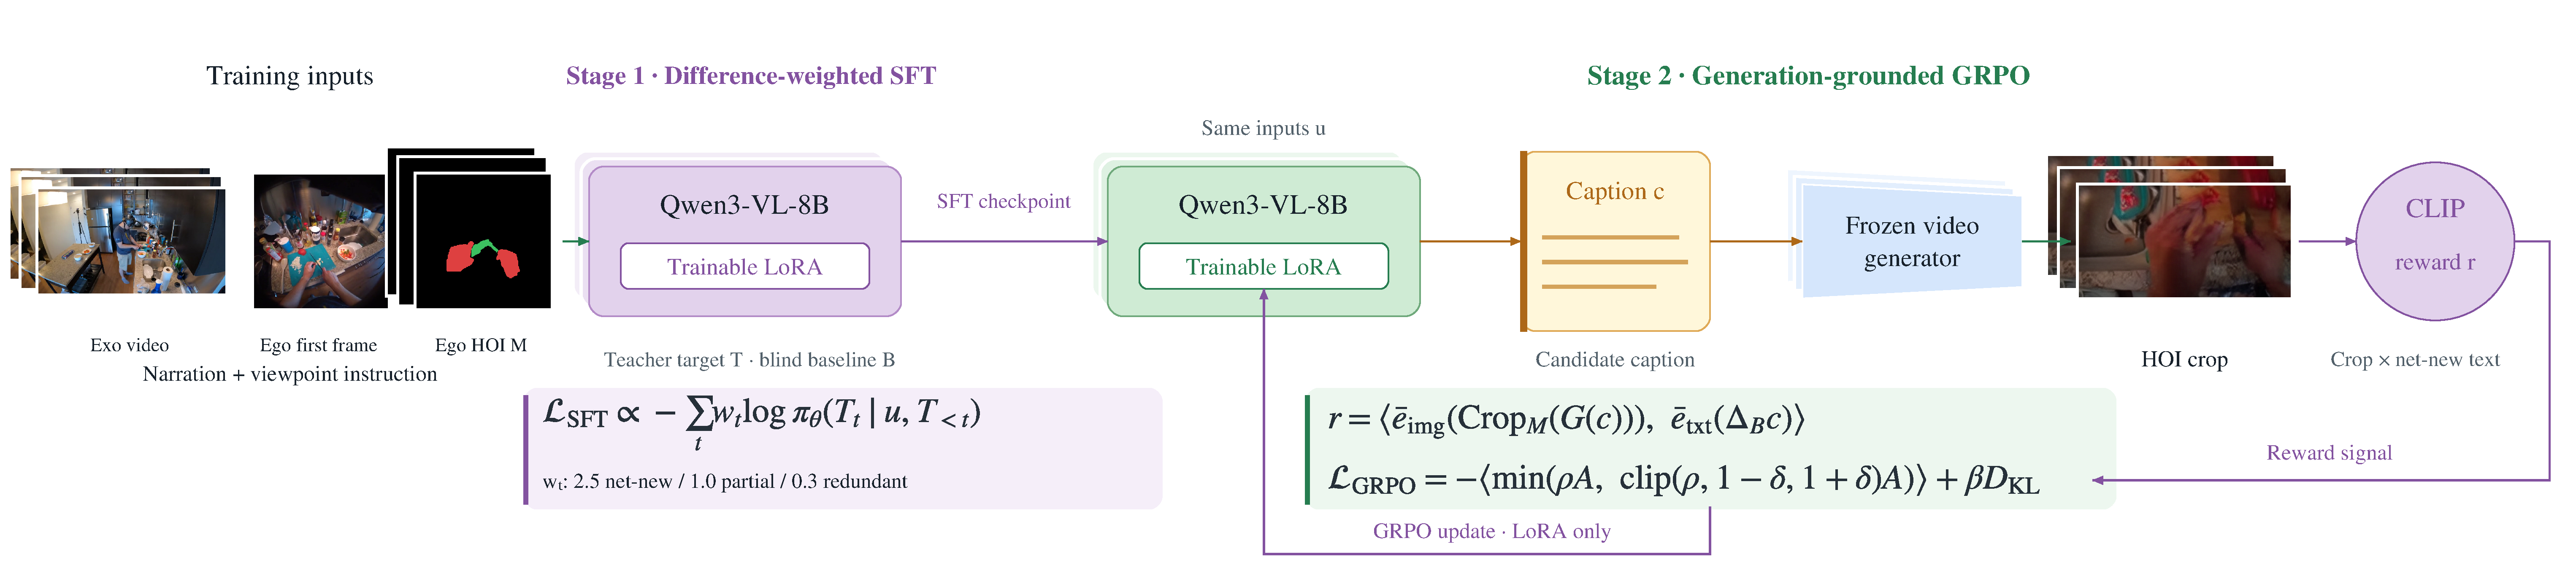
\includegraphics[width=\textwidth]{figs/qwen_architecture.pdf}
\caption{\textbf{Training the Qwen cross-view caption converter.}
Difference-weighted SFT fits offline teacher captions under
Eq.~\ref{eq:caption-sft}. GRPO then samples captions, renders previews with
a frozen generator, and uses the local CLIP reward in
Eq.~\ref{eq:caption-reward} to update the converter with GRPO. Only the converter's LoRA parameters are optimized.}
\label{fig:any2ego_qwen}
\end{figure*}

\subsection{Spatial and semantic condition injection}
\label{sec:condition-injection}
\label{sec:stage1-method}
\label{sec:stage2-method}
\label{sec:spatial-route}

The predicted HOI masks $M$ enter Wan2.1-VACE through its 15-block control
branch. Its layer-wise features are added to the hidden video tokens with
control strength $\lambda_M$. The ego first frame $I_0$ provides the image
condition, and narration $n$ uses the native text-conditioning path.

The Qwen caption $c$ is encoded by frozen umT5 into $E_c$. We add a caption
cross-attention branch to each of the 30 main-Transformer blocks, reusing its
video queries $Q^{(\ell)}$ and learning caption key/value projections:
\begin{equation}
K_c^{(\ell)}=E_cW_{K,c}^{(\ell)},\quad
V_c^{(\ell)}=E_cW_{V,c}^{(\ell)},\quad
A_c^{(\ell)}=\operatorname{softmax}\!\left(
\frac{Q^{(\ell)}(K_c^{(\ell)})^\top}{\sqrt d}\right)V_c^{(\ell)}.
\label{eq:caption-attention}
\end{equation}
Here $d$ is the attention head dimension. Caption attention is weighted and
added to the native narration/image attention $A_{\mathrm{native}}$ before
the frozen output projection:
\begin{equation}
\begin{aligned}
O_i^{(\ell)} &= W_O^{(\ell)}\!\left[
A_{\mathrm{native},i}^{(\ell)}+g^{(\ell)}s_i^{(\ell)}A_{c,i}^{(\ell)}\right],\\
s_i^{(\ell)}&=
\begin{cases}
1, & \text{global gate},\\
\sigma\!\left((w^{(\ell)})^\top\operatorname{sg}(m_i)+b^{(\ell)}\right),
& \text{spatial routing}.
\end{cases}
\end{aligned}
\label{eq:caption-injection}
\end{equation}
The spatial variant uses the VACE branch's pre-block HOI features $m_i$,
aligned with video token $i$; $\operatorname{sg}$ stops gradients and
$\sigma$ is sigmoid. We initialize $g^{(\ell)}=0.1$ and $w^{(\ell)}=b^{(\ell)}=0$,
so the spatial factor initially equals $0.5$. Setting $g^{(\ell)}=0$ removes
the caption contribution.

Training first fits rank-128 LoRA on the VACE control branch with the main
backbone frozen. It then freezes this spatial branch and optimizes the
caption projections and gate, using caption dropout. Both stages use the
backbone's flow-matching loss:
\begin{equation}
\mathcal L_{\mathrm{video}}(\psi)=
\mathbb E_{z,\epsilon_z,\tau}\!\left[
\omega(\tau)\operatorname{MSE}\!\left(
P_+v_\psi(z_\tau,\tau;\mathcal C),\,P_+(\epsilon_z-z)\right)\right].
\label{eq:video-training}
\end{equation}
Here $z_\tau=(1-\tau)z+\tau\epsilon_z$, $z$ is the encoded ego video,
$\epsilon_z$ is Gaussian noise, and $\omega(\tau)$ is the scheduler weight.
$P_+$ excludes the fixed first latent frame. Conditions $\mathcal C$ are
$(I_0,M,n)$ in Stage 1 and $(I_0,M,n,c)$ in Stage 2; $\psi$ denotes the
parameters trained in the corresponding stage.

\section{Experiments}
\label{sec:setup}
\label{sec:results}

\textbf{Dataset.} We evaluate Any2Ego on cooking clips from Ego-Exo4D
\citep{grauman2024egoexo4d}. The
training set comprises 34{,}242 annotated clips. For evaluation we use a
randomly sampled, disjoint-from-training $N=1{,}000$ test pool of EgoExo4D
clips passed through the same HOI-mask annotation and deployable-caption
pipeline; all three checkpoints (mask-only base, global-gate caption,
spatial-route caption) produced predictions at $480\times480$ with matched
inference settings, evaluated against the real future ego frames, on this
shared pool. Construction, caption provenance, and interpretation are defined
in one place, Section~\ref{sec:stage2}.

\textbf{Evaluation metrics.}
\label{sec:metrics}
We report SSIM and PSNR ($\uparrow$), LPIPS ($\downarrow$), and FVD
($\downarrow$). Frame-level metrics measure visual agreement with the ego
reference, while FVD measures mismatch between video-feature distributions.
Short clips can retain much of their first-frame appearance, so we read
frame-level scores together with FVD. Additional temporal diagnostics are
in Appendix~\ref{app:results-detail}.

We first evaluate caption quality, then compare injection strategies and
analyze routing. We next compare continuous VLM features with text,
followed by open-source baselines and condition-content ablations.

\subsection{Caption quality evaluation}
\label{sec:captioner-eval}
\label{sec:media-judge}

Caption-quality evaluation complements the downstream video-generation
results. On the same $N{=}1{,}000$ clips, Qwen3.5-27B judges each caption
against $13$ ground-truth ego frames, scoring six semantic fields and overall
faithfulness from $1$ to $5$, together with a grammaticality flag.
We report the mean field score (label-mean), overall, and a composite score
that subtracts penalties for rule-zero and grammar failures.
Rule-zero flags explicit mentions of recording equipment.
All models receive the same inference-time inputs and post-processing.

Table~\ref{tab:media-judge} shows that our converter achieves the highest
composite ($4.043$), overall ($4.051$), and label-mean ($4.281$), exceeding the
strongest off-the-shelf VLM by $0.915$ composite. SFT raises label-mean from
$3.164$ to $4.160$; adding GRPO increases it to $4.281$ and composite from
$3.689$ to $4.043$. The judge's grammar pass rate on post-processed captions
is $68.2\%$ for SFT and $97.5\%$ after GRPO. Our converter leads in four of
the six semantic fields; per-field results and the distinction between
grammar scoring and output-format completeness are given in
Appendix~\ref{app:results-detail}.

\begin{table}[h]
\centering
\footnotesize
\captionsetup{font=footnotesize}
\caption{Caption quality on $N{=}1{,}000$ clips, evaluated by Qwen3.5-27B.
Label-mean averages six field scores; $\mathrm{Comp.}=\mathrm{Overall}
-\mathbb{1}[\mathrm{Rule\mbox{-}0}]-0.3\mathbb{1}[\neg\mathrm{Gram.}]$.
Gram. is the judge's pass rate on post-processed captions.
Higher is better except Rule-0. Best per column in \textbf{bold}.}
\label{tab:media-judge}
\resizebox{\linewidth}{!}{%
\begin{tabular}{llrrrrr}
\toprule
Caption source & Backbone & Comp.\ $\uparrow$ & Overall $\uparrow$ & Label-mean $\uparrow$ & Rule-0 $\downarrow$ & Gram.\ $\uparrow$ \\
\midrule
\textbf{Ours (converter, SFT\,+\,GRPO)} & Qwen3-VL-8B & \textbf{4.043} & \textbf{4.051} & \textbf{4.281} & 0.0\% & 97.5\% \\
\;\; before GRPO (SFT only)             & Qwen3-VL-8B & 3.689 & 3.790 & 4.160 & 0.6\% & 68.2\% \\
\midrule
Qwen3-VL-32B  & 32B  & 3.128 & 3.131 & 3.529 & 0.0\% & 99.1\% \\
Qwen3-VL-235B & 235B & 3.079 & 3.079 & 3.430 & 0.0\% & \textbf{99.9\%} \\
Qwen3.5-9B    & 9B   & 3.003 & 3.004 & 3.354 & 0.0\% & 99.8\% \\
Qwen3-VL-8B   & 8B   & 2.829 & 2.831 & 3.164 & 0.0\% & 99.3\% \\
\bottomrule
\end{tabular}%
}
\end{table}

Per-field scores (Table~\ref{tab:media-judge-fields}) are in
Appendix~\ref{app:results-detail}.

\subsection{Comparison of condition-injection strategies}
\label{sec:stage1}
\label{sec:stage2}

With the predicted HOI masks $M$ and the Qwen-generated caption $c$
available, we compare three generator variants using the injection designs
in Section~\ref{sec:condition-injection}. \textbf{HOI-only} uses the mask
control branch without the additional caption branch. \textbf{Global}
adds caption cross-attention with one learned scalar gate per block.
\textbf{Spatial} further modulates that branch at each video token using
aligned HOI features. Global and Spatial receive identical captions for
each clip; all three share the ego first frame, masks, and task narration.

We first train the HOI-only model by adapting the VACE control branch with
LoRA. Global and Spatial start from this same checkpoint, freeze the
backbone and trained control branch, and train only the added caption
branch and its gates using the flow-matching objective in
Eq.~\ref{eq:video-training}. The Qwen converter is fixed during this
comparison. We evaluate the three trained variants on the same $N{=}1{,}000$
EgoExo4D cooking clips randomly sampled from the held-out test data,
disjoint from training, at
$480\times480$ with matched frame counts and inference settings.
Checkpoint and evaluation details are in Appendix~\ref{app:results-detail}.

Table~\ref{tab:phase2-testpool} reports the results. Adding Global caption
injection raises SSIM from $0.6084$ to $0.6358$ and reduces FVD from
$42.63$ to $37.76$. Spatial further improves SSIM to $0.6603$, PSNR to
$22.28$\,dB, LPIPS to $0.1440$, and FVD to $33.34$. Relative to HOI-only,
Spatial reduces LPIPS by $25.7\%$ and FVD by $21.8\%$; its FVD is also
$11.7\%$ lower than Global. These are aggregate results on this evaluation
pool, rather than a claim that every individual clip improves.

\begin{table}[h]
\centering
\footnotesize
\captionsetup{font=footnotesize}
\caption{Condition-injection comparison on the same $N{=}1{,}000$ clips.
All variants share the HOI-conditioned base; Global and Spatial use the
same Qwen captions. Resolution and inference settings are matched.
Best values are in \textbf{bold}.}
\label{tab:phase2-testpool}
\begin{tabular}{lrrrr}
\toprule
Method & SSIM $\uparrow$ & PSNR $\uparrow$ & LPIPS $\downarrow$ & FVD $\downarrow$ \\
\midrule
HOI-only & 0.6084 & 21.06 & 0.1937 & 42.63 \\
Global & 0.6358 & 21.74 & 0.1631 & 37.76 \\
Spatial (ours) & \textbf{0.6603} & \textbf{22.28} & \textbf{0.1440} & \textbf{33.34} \\
\bottomrule
\end{tabular}
\end{table}

Figure~\ref{fig:qual-compare} places the three generated outputs side by
side with the corresponding ground-truth frames. The examples show
differences in viewpoint-dependent scene layout during skillet placement,
overhead-cabinet appearance when scooping oil, and window/background
content in the milk-tea-cup clip. The full-frame grid exposes layout changes
and local appearance differences. Spatial better preserves the
illustrated structures, motivating the routing analysis below.

\begin{figure*}[t]
\centering
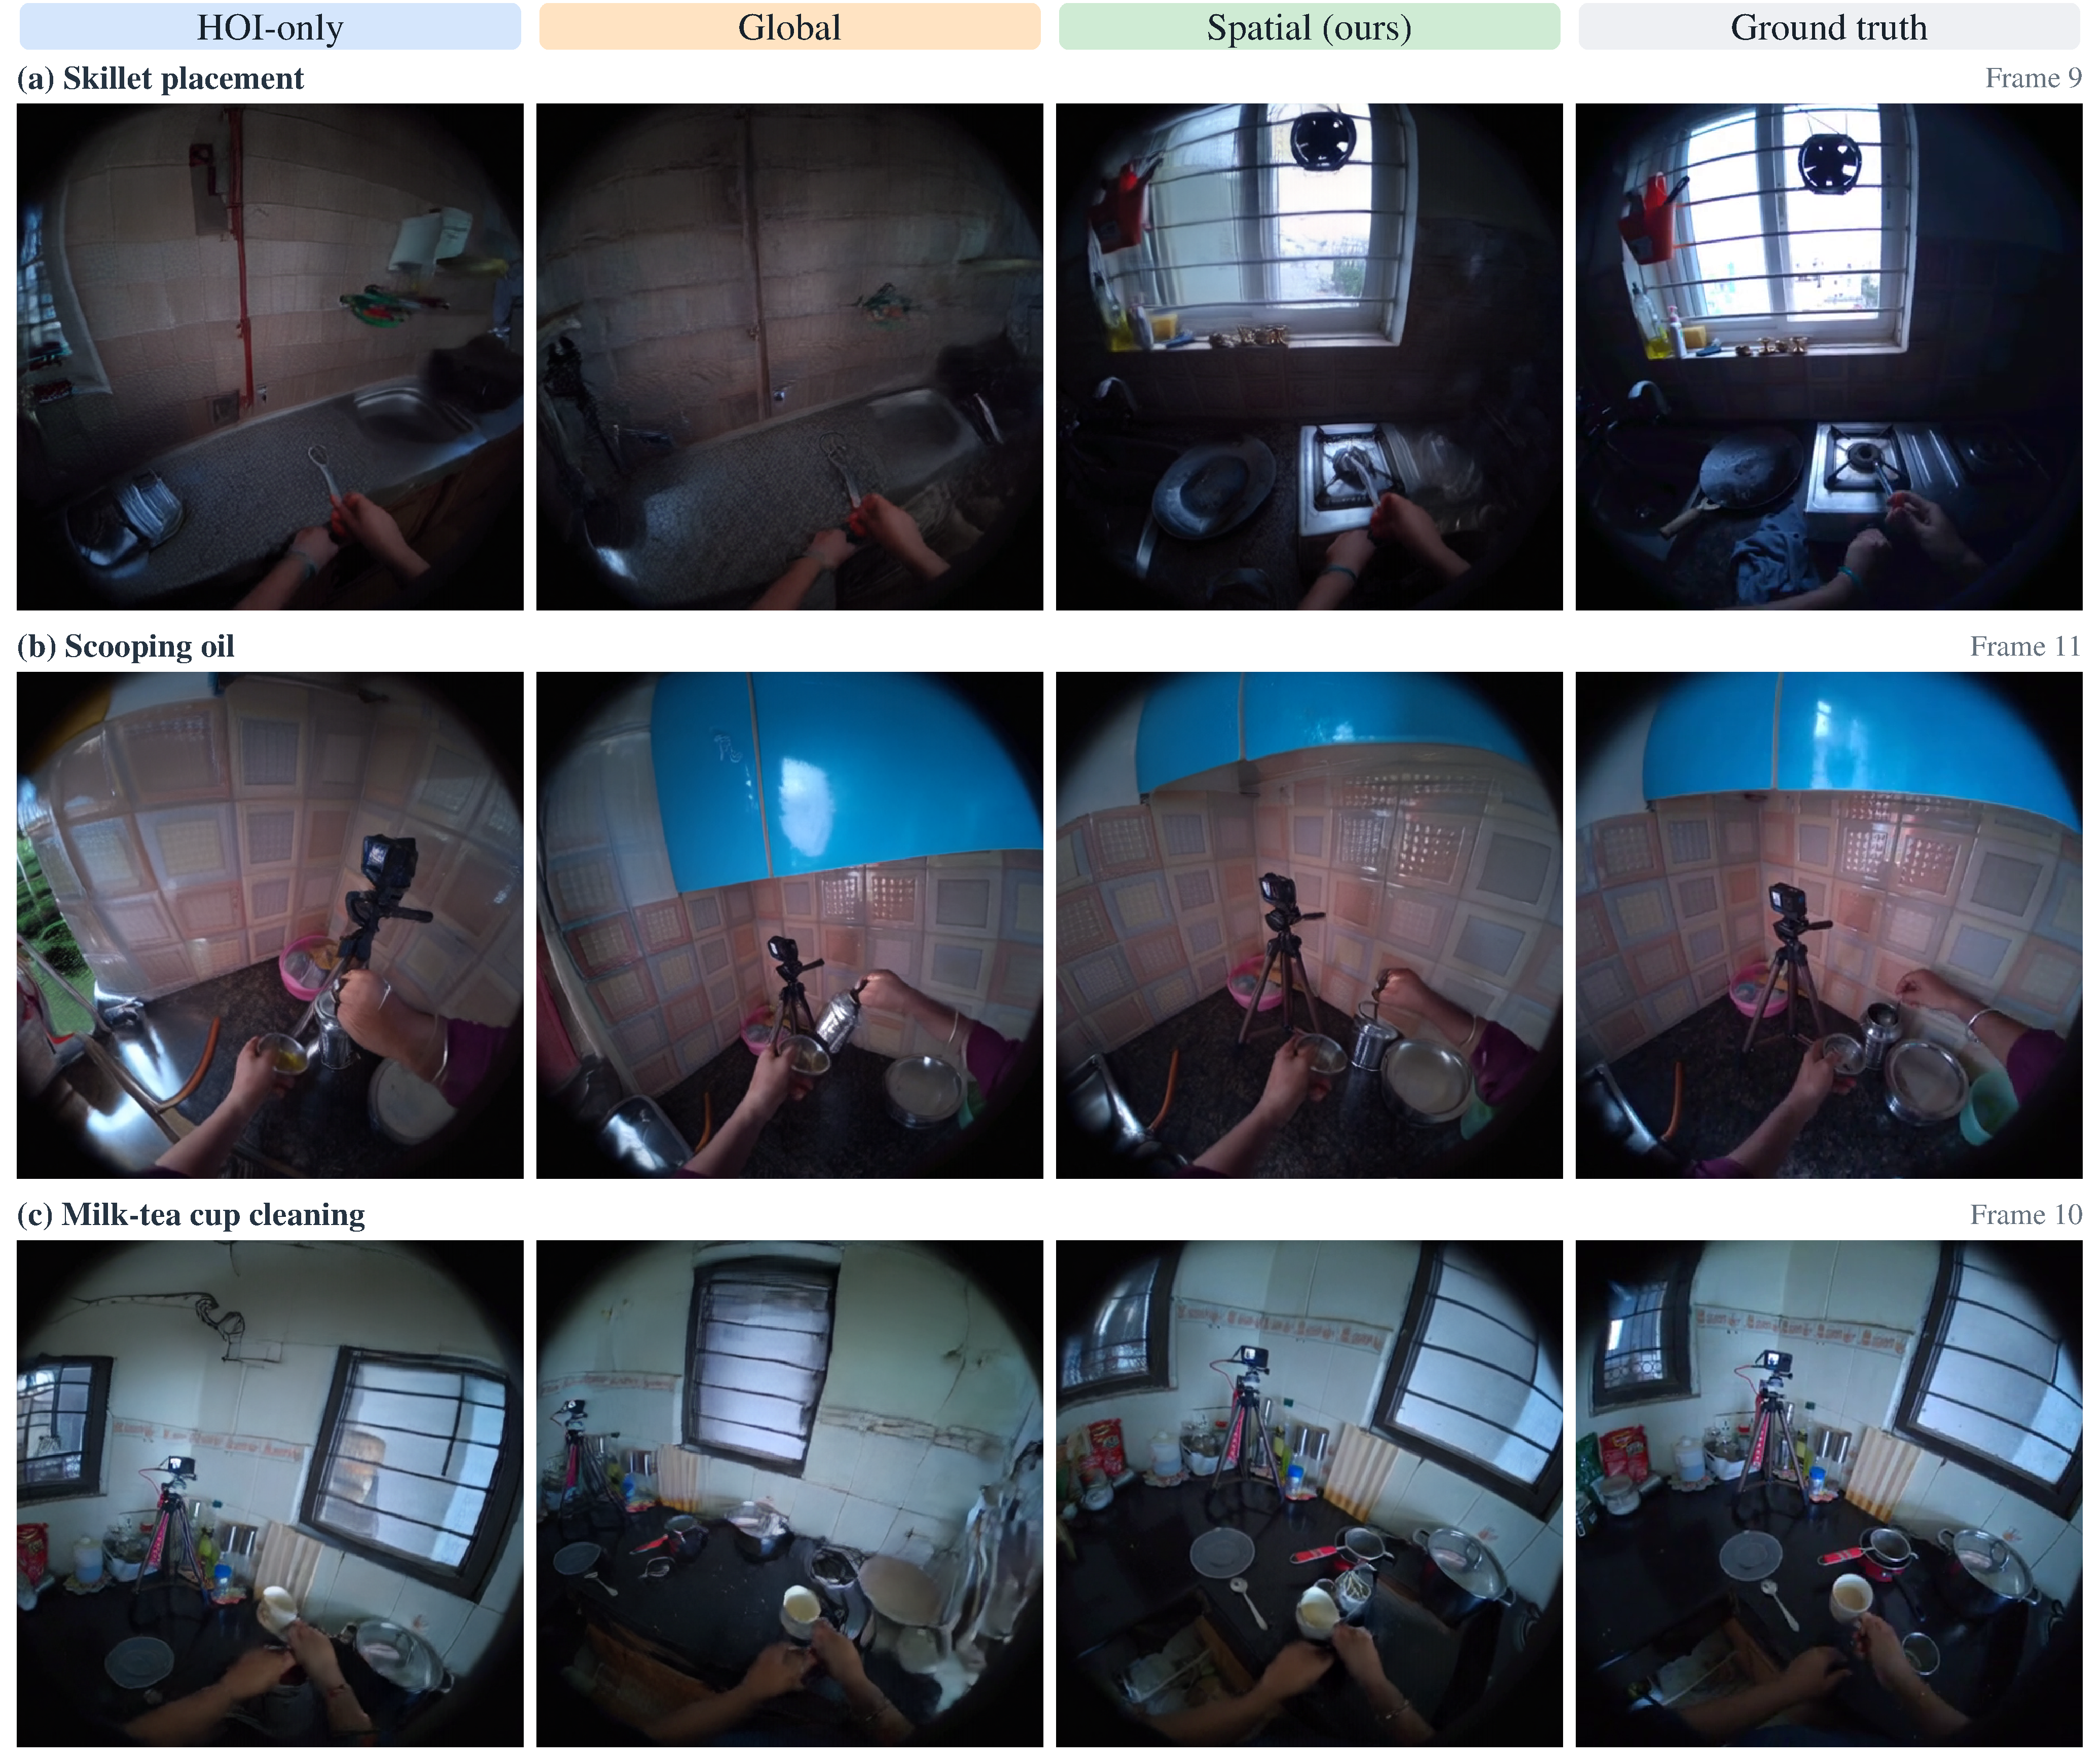
\includegraphics[width=\textwidth]{figs/qual_compare/qualitative_grid.pdf}
\caption{\textbf{Qualitative comparison of the three injection strategies.}
HOI-only, Global, and Spatial outputs are shown alongside ground truth for
(a) skillet placement, frame 9; (b) scooping oil, frame 11; and
(c) cleaning a milk-tea cup, frame 10. Each row shows four full frames at
the same time index. All examples belong to the
$N{=}1{,}000$ evaluation pool; ground truth is shown only for comparison.}
\label{fig:qual-compare}
\end{figure*}

\subsection{Why spatial injection can improve generation}
\label{sec:diagnosis}

Global already produces token-dependent caption attention: the video
queries in Eq.~\ref{eq:caption-attention} differ across locations.
Its limitation is the shared \emph{scaling} of those responses within a
block. Spatial adds an HOI-conditioned scale, allowing different locations
to receive different correction strengths. To make this distinction
explicit, consider one block at one denoising step and hold its attention
responses fixed. Let $a_i=W_O A_{c,i}$ be the projected caption response
at token $i$, and let $r_i$ be a desired local correction to the
HOI-only representation. A quadratic approximation gives
\begin{equation}
\mathcal E_G(g)=\sum_i\|r_i-ga_i\|_2^2,\qquad
\mathcal E_S(g,s)=\sum_i\|r_i-gs_i a_i\|_2^2.
\label{eq:routing-local-error}
\end{equation}
Minimizing the global error gives
$g_G^*=\sum_i a_i^\top r_i/\sum_i\|a_i\|_2^2$.
Thus one gate must balance locations that need a correction against
locations where the same branch response is unnecessary or inconsistent.
For an illustrative case, suppose $r_i=\kappa a_i$ on a relevant token set
$\mathcal F$ and $r_i=0$ elsewhere, with $\kappa>0$. Define response energies
$E_{\mathcal F}=\sum_{i\in\mathcal F}\|a_i\|_2^2$ and
$E_{\overline{\mathcal F}}=\sum_{i\notin\mathcal F}\|a_i\|_2^2$. Then
\begin{equation}
g_G^*=\kappa\frac{E_{\mathcal F}}
{E_{\mathcal F}+E_{\overline{\mathcal F}}},\qquad
\mathcal E_G(g_G^*)=\kappa^2
\frac{E_{\mathcal F}E_{\overline{\mathcal F}}}
{E_{\mathcal F}+E_{\overline{\mathcal F}}}.
\label{eq:routing-dilution}
\end{equation}
An ideal spatial scale approaching $1$ on $\mathcal F$ and $0$ elsewhere
can instead approach zero error in this example with $g=\kappa$.
The implemented sigmoid gate only approximates such spatial selectivity;
its success depends on what the HOI features and training can identify.

Here relevance is caption-dependent: $\mathcal F$ need not coincide with
the hand/object foreground, because captions also describe scene and
lighting. The route uses HOI features to adjust semantic influence by location,
while subsequent Transformer layers propagate local changes across the
scene. This explains how spatially selective updates can support the layout
and appearance improvements in Figure~\ref{fig:qual-compare}.

\subsection{Text captions versus continuous VLM features}
\label{sec:modality-eval}

We next compare two ways of carrying semantic information across views.
The continuous branch extracts visual and instruction tokens from layer 32
of frozen Qwen3-VL-32B using 13 exo frames, projects the 5120-dimensional
features into the video model, and injects them through a globally gated
cross-attention branch. The text branch uses the converter's first-person
caption encoded by umT5. Both use the same trained HOI-conditioned base,
with that base frozen while the added branch is trained, and the same
$480\times480$, 13-frame evaluation on $N{=}1{,}000$ clips.
The Global text row is the closest gating comparison; Spatial additionally
uses the routing mechanism analyzed in Section~\ref{sec:diagnosis}.

\begin{table}[h]
\centering
\footnotesize
\caption{Intermediate-conditioning comparison on $N{=}1{,}000$ clips.
All rows share the HOI-conditioned base and evaluation settings.
Global gating compares the two semantic paths; Spatial adds HOI-guided routing.}
\label{tab:modality}
\begin{tabular}{lrrrr}
\toprule
Conditioning path & SSIM $\uparrow$ & PSNR $\uparrow$ & LPIPS $\downarrow$ & FVD $\downarrow$ \\
\midrule
HOI-only & 0.6084 & 21.06 & 0.1937 & 42.63 \\
VLM features, global gate & 0.6181 & 21.22 & 0.1838 & 44.52 \\
Text caption, Global & 0.6358 & 21.74 & 0.1631 & 37.76 \\
Text caption, Spatial & \textbf{0.6603} & \textbf{22.28} & \textbf{0.1440} & \textbf{33.34} \\
\bottomrule
\end{tabular}
\end{table}

The completed VLM inference improves frame-level scores over HOI-only,
but trails both text variants (Table~\ref{tab:modality}); its FVD of
$44.52$ also provides no distributional improvement over the base.
Even without spatial routing, text raises SSIM by $0.0177$ and reduces
LPIPS by $0.0207$ relative to continuous features.
Thus the observed text advantage is already present under global gating.

The result is consistent with three advantages of our caption pathway.
First, the converter selects interaction-relevant information---hands,
objects, contact, motion, scene, and lighting---instead of passing all exo
appearance features to the generator. Second, its supervision explicitly
expresses that information from the target first-person viewpoint. The
continuous branch retains source-view hidden tokens, so its projection and
attention layers must also learn how those tokens relate to the ego scene.
Third, umT5 encodes the caption in the text representation already used by
the video backbone. This combination of semantic selection, viewpoint
conversion, and text-space compatibility gives the generator a more directly
usable condition; HOI-guided spatial routing then determines where to apply
it.

\subsection{Comparison with open-source video generators}
\label{sec:opensource-baselines}

Table~\ref{tab:opensource-baselines} compares the same $N{=}1{,}000$ clips
with open-source generators. V2V models receive the exo video; I2V/TI2V
models receive the ego first frame and, where supported, the original task
prompt. Stable Video Diffusion is image-only. We report only these native
input settings here. In particular, I2V/TI2V models have no exo observation
from which to recover the demonstrated action or its target viewpoint.
Resolution and scoring are shared; model-specific settings are in
Appendix~\ref{app:results-detail}.

\begin{table}[h]
\centering
\footnotesize
\caption{Open-source generator comparison on $N{=}1{,}000$ clips.
Text-capable I2V models use the task prompt; SVD uses only the ego first
frame. All results use the same evaluation pipeline.}
\label{tab:opensource-baselines}
\begin{tabular}{llrrrr}
\toprule
Method & Sees exo & SSIM $\uparrow$ & PSNR $\uparrow$ & LPIPS $\downarrow$ & FVD $\downarrow$ \\
\midrule
Wan2.1-VACE-1.3B (vanilla) & yes & 0.178 & 10.14 & 0.711 & 1118.7 \\
Wan2.1-Fun-1.3B-Control & yes & 0.368 & 12.30 & 0.844 & 2361.1 \\
\midrule
Wan2.2-TI2V-5B + prompt & no & 0.553 & 20.74 & 0.225 & 127.6 \\
LTX-Video + prompt & no & 0.574 & 20.85 & 0.210 & 121.6 \\
CogVideoX-5B-I2V + prompt & no & 0.578 & 21.09 & 0.211 & 148.3 \\
Stable Video Diffusion & no & 0.438 & 16.10 & 0.386 & 177.0 \\
\midrule
HOI-only & yes & 0.608 & 21.06 & 0.194 & 42.6 \\
Spatial (ours) & yes & \textbf{0.660} & \textbf{22.28} & \textbf{0.144} & \textbf{33.3} \\
\bottomrule
\end{tabular}
\end{table}

I2V baselines obtain FVD scores of $121.6$--$177.0$, compared with our
$33.3$. Their first-frame condition provides scene appearance but leaves
the demonstrated action and viewpoint evolution underconstrained. On these
short clips, preserving the initial appearance can yield competitive
frame-level scores while missing the actual temporal changes. Higher FVD
reflects the remaining mismatch in video appearance and motion together.
Our predicted HOI geometry and first-person captions provide complementary
constraints on both the interaction and its evolution. The V2V results
likewise show that raw exo imagery alone does not resolve the viewpoint gap;
model-specific input conventions are documented in the appendix.

\subsection{Condition-content ablation}
\label{sec:component-ablation}

We test whether the trained Spatial model uses the content of each anchor
by randomizing one inference condition while keeping the other and all
model weights fixed. Caption randomization preserves text length; mask
randomization preserves the per-class pixel budget while changing spatial
locations. Table~\ref{tab:component-ablation} reports all three conditions
on the same $N{=}1{,}000$ clips.

\begin{table}[h]
\centering
\footnotesize
\captionsetup{font=footnotesize}
\caption{Condition-content ablation on $N{=}1{,}000$ clips. We keep the trained
Spatial model fixed and randomize one condition at a time. Full wins is the
fraction of clips where the original conditions yield higher SSIM than the
corresponding randomized input.}
\label{tab:component-ablation}
\begin{tabular}{lrrrr}
\toprule
Arm & PSNR $\uparrow$ & SSIM $\uparrow$ & LPIPS $\downarrow$ & Full wins (SSIM) \\
\midrule
\textbf{Full (original conditions)} & \textbf{22.284} & \textbf{0.6603} & \textbf{0.1440} & -- \\
cap\_random (caption $\to$ random text) & 21.586 & 0.6315 & 0.1661 & $88.7\%$ \\
mask\_random (mask $\to$ random position) & 16.379 & 0.4234 & 0.5042 & $100.0\%$ \\
\bottomrule
\end{tabular}
\end{table}

Randomizing captions reduces SSIM from $0.6603$ to $0.6315$ and increases
LPIPS from $0.1440$ to $0.1661$; the original conditions win on $88.7\%$
of clips. Randomizing masks has a larger effect ($0.4234$ SSIM,
$0.5042$ LPIPS), with the original conditions winning on every evaluated
clip. The spatial anchor therefore provides the stronger geometric
constraint, while caption content contributes additional semantic guidance.
These are inference-time content perturbations, not separately retrained
branch-removal models; the full protocol is in
Appendix~\ref{app:results-detail}.

\subsection{Test-set coverage and score distributions}
\label{sec:coverage-compute}
The $1{,}000$ evaluation clips have unique clip identifiers and span
281 takes, 47 physical settings, 13 cooking tasks, and 10 collecting
institutions in the EgoExo4D metadata. The source takes do not overlap
with those in the Stage 1 and Stage 2 generator training manifests.
These statistics characterize the split and its coverage within cooking;
the counting protocol is given in Appendix~\ref{app:results-detail}.

Figure~\ref{fig:metric-distributions} shows the full per-clip SSIM and PSNR
distributions. For HOI-only, Global, and Spatial, median SSIM is
$0.613/0.638/0.657$ and median PSNR is $21.27/21.80/22.35$ dB.
These summaries complement the mean scores in
Table~\ref{tab:phase2-testpool} by describing the center and spread of
the evaluated score distributions.

\section{Conclusion}
\label{sec:conclusion}

We set out to make exo-to-ego video generation easier by inserting an
intermediate hand--object modality -- a spatial layer (HOI mask) and a
semantic layer (ego-perspective caption) -- between the two views. On our
fixed $N{=}1{,}000$ EgoExo4D test pool, scored with deployable captions,
the two layers stack constructively: adding the caption layer improves every
metric monotonically, base $\to$ global gate $\to$ spatial route
(Table~\ref{tab:phase2-testpool}). We traced this to a fixable mechanism -- a
global scalar gate that dilutes the caption's localized signal across
mostly-static tokens -- and fixed it with a per-token spatial route reusing
the model's own HOI-mask features, which is best on every metric, as the
routing argument predicts. Both halves of the
intermediate modality are produced, not assumed -- the spatial anchor by
$\Phi_{\text{seg}}$ (Section~\ref{sec:phiseg-method}), the textual anchor by a
distilled, RL-refined captioner (Section~\ref{sec:captioner-eval}) -- so no
component reads the ground-truth ego video at inference. The broader
message: an intermediate modality turns one hard cross-view mapping into two
easier, separately inspectable ones, which is what let us localize where the
remaining signal is lost.

\section{Limitations}

We use a different diffusion backbone (Wan2.1-VACE) than the original
EgoExo-Gen paper \citep{xu2025egoexogen} (SEINE), so the corresponding
experiments are internally controlled comparisons rather than a direct
head-to-head reproduction of that method. Our evaluation covers a randomly
sampled, fixed pool of $1{,}000$ EgoExo4D cooking clips, disjoint from
training; generalization to other activities and datasets remains a separate
question. All compared methods use the same evaluation pool.

\section*{Reproducibility Statement}
All training and evaluation scripts referenced in this paper (data
construction, Stage 1/2 training and
inference, the routing analysis of Section~\ref{sec:diagnosis}, and the
$\Phi_{\text{seg}}$/GRPO code of Sections~\ref{sec:phiseg-method}
and~\ref{sec:student-method}) are implemented in
the accompanying code release. Table~\ref{tab:phase2-testpool} reports the exact
clip counts for the fixed $N=1{,}000$ test pool used throughout,
with all metrics computed under one shared frame-loading pipeline.

\section*{Ethics Statement}
This work uses only the existing, publicly documented EgoExo4D dataset of
cooking activities, released for research use; we introduce no new human
data collection. The generative model studied here is scoped to short
kitchen-activity clips and is not evaluated for, and we do not recommend its
use for, generating egocentric video of individuals without consent or in
safety-, privacy-, or identity-sensitive contexts.

\bibliographystyle{iclr2027_conference}
\begin{thebibliography}{99}

\bibitem[Blattmann et al.(2023)]{blattmann2023svd}
A.\ Blattmann, T.\ Dockhorn, S.\ Kulal, D.\ Mendelevitch, M.\ Kilian,
D.\ Lorenz, Y.\ Levi, Z.\ English, V.\ Voleti, A.\ Letts, V.\ Jampani, and
R.\ Rombach.
\newblock Stable Video Diffusion: Scaling Latent Video Diffusion Models to
Large Datasets.
\newblock \emph{arXiv preprint arXiv:2311.15127}, 2023.

\bibitem[Cheng et al.(2023)]{cheng2023hands23}
T.\ Cheng, D.\ Shan, A.\ Hassen, R.\ Higgins, and D.\ Fouhey.
\newblock Towards A Richer 2D Understanding of Hands at Scale (hands23).
\newblock \emph{NeurIPS}, 2023.

\bibitem[Cheng \& Schwing(2022)]{cheng2022xmem}
H.\ K.\ Cheng and A.\ G.\ Schwing.
\newblock XMem: Long-Term Video Object Segmentation with an Atkinson-Shiffrin
Memory Model.
\newblock \emph{ECCV}, 2022.

\bibitem[Grauman et al.(2024)]{grauman2024egoexo4d}
K.\ Grauman, et al.
\newblock Ego-Exo4D: Understanding Skilled Human Activity from First- and
Third-Person Views.
\newblock \emph{CVPR}, 2024.

\bibitem[Liu et al.(2023)]{liu2023groundingdino}
S.\ Liu, Z.\ Zeng, T.\ Ren, F.\ Li, H.\ Zhang, J.\ Yang, C.\ Li, J.\ Yang,
H.\ Su, J.\ Zhu, and L.\ Zhang.
\newblock Grounding DINO: Marrying DINO with Grounded Pre-Training for
Open-Set Object Detection.
\newblock \emph{arXiv preprint arXiv:2303.05499}, 2023.

\bibitem[Oh et al.(2019)]{oh2019stm}
S.\ W.\ Oh, J.-Y.\ Lee, N.\ Xu, and S.\ J.\ Kim.
\newblock Video Object Segmentation using Space-Time Memory Networks.
\newblock \emph{ICCV}, 2019.

\bibitem[Peebles \& Xie(2023)]{peebles2023dit}
W.\ Peebles and S.\ Xie.
\newblock Scalable Diffusion Models with Transformers.
\newblock \emph{ICCV}, 2023.

\bibitem[Ravi et al.(2024)]{ravi2024sam2}
N.\ Ravi, V.\ Gabeur, Y.-T.\ Hu, R.\ Hu, C.\ Ryali, T.\ Ma, H.\ Khedr,
R.\ R\"adle, C.\ Rolland, L.\ Gustafson, E.\ Mintun, J.\ Pan, K.\ V.\ Alwala,
N.\ Carion, C.-Y.\ Wu, R.\ Girshick, P.\ Doll\'ar, and C.\ Feichtenhofer.
\newblock SAM 2: Segment Anything in Images and Videos.
\newblock \emph{arXiv preprint arXiv:2408.00714}, 2024.

\bibitem[Radford et al.(2021)]{radford2021clip}
A.\ Radford, J.\ W.\ Kim, C.\ Hallacy, A.\ Ramesh, G.\ Goh, S.\ Agarwal,
G.\ Sastry, A.\ Askell, P.\ Mishkin, J.\ Clark, G.\ Krueger, and I.\ Sutskever.
\newblock Learning Transferable Visual Models From Natural Language Supervision.
\newblock \emph{ICML}, 2021.

\bibitem[Ren et al.(2024)]{ren2024consisti2v}
Y.\ Ren, Y.\ Zhou, J.\ Yang, J.\ Shi, D.\ Liu, F.\ Zhang, M.\ Wang, and
X.\ Chen.
\newblock ConsistI2V: Enhancing Visual Consistency for Image-to-Video
Generation.
\newblock \emph{arXiv preprint arXiv:2402.04324}, 2024.

\bibitem[Yang et al.(2024)]{yang2024cogvideox}
Z.\ Yang, J.\ Teng, W.\ Zheng, M.\ Ding, S.\ Huang, J.\ Xu, Y.\ Yang, W.\ Hong,
X.\ Zhang, G.\ Feng, et al.
\newblock CogVideoX: Text-to-Video Diffusion Models with An Expert
Transformer.
\newblock \emph{arXiv preprint arXiv:2408.06072}, 2024.

\bibitem[HaCohen et al.(2025)]{hacohen2025ltxvideo}
Y.\ HaCohen, N.\ Chiprut, B.\ Brazowski, D.\ Shalem, D.\ Moshe, E.\ Richardson,
E.\ Levin, G.\ Shiran, N.\ Zabari, O.\ Gordon, et al.
\newblock LTX-Video: Realtime Video Latent Diffusion.
\newblock \emph{arXiv preprint arXiv:2501.00103}, 2025.

\bibitem[Shao et al.(2024)]{shao2024grpo}
Z.\ Shao, P.\ Wang, Q.\ Zhu, R.\ Xu, J.\ Song, M.\ Zhang, Y.\ K.\ Li, Y.\ Wu,
and D.\ Guo.
\newblock DeepSeekMath: Pushing the Limits of Mathematical Reasoning in Open
Language Models.
\newblock \emph{arXiv preprint arXiv:2402.03300}, 2024.

\bibitem[Wan et al.(2025)]{wan2025}
Team Wan, A.\ Wang, B.\ Ai, B.\ Wen, C.\ Mao, C.-W.\ Xie, D.\ Chen, F.\ Yu,
H.\ Zhao, J.\ Yang, et al.
\newblock Wan: Open and Advanced Large-Scale Video Generative Models.
\newblock \emph{arXiv preprint arXiv:2503.20314}, 2025.

\bibitem[Jiang et al.(2025)]{vace2025}
Z.\ Jiang, Z.\ Han, C.\ Mao, J.\ Zhang, Y.\ Pan, and Y.\ Liu.
\newblock VACE: All-in-One Video Creation and Editing.
\newblock \emph{arXiv preprint arXiv:2503.07598}, 2025.

\bibitem[Xu et al.(2025)]{xu2025egoexogen}
J.\ Xu, Y.\ Huang, B.\ Pei, J.\ Hou, Q.\ Li, G.\ Chen, Y.\ Zhang, R.\ Feng, and
W.\ Xie.
\newblock EgoExo-Gen: Ego-centric Video Prediction by Watching Exo-centric
Videos.
\newblock \emph{ICLR}, 2025.

\bibitem[Kang et al.(2025)]{kang2025egox}
T.\ Kang, K.\ Kim, D.\ Kim, M.\ Park, J.\ Hyung, and J.\ Choo.
\newblock EgoX: Egocentric Video Generation from a Single Exocentric Video.
\newblock \emph{arXiv preprint arXiv:2512.08269}, 2025.

\end{thebibliography}

\appendix

This appendix provides training settings
(Appendix~\ref{app:impl}), caption-injection settings
(Appendix~\ref{app:code}), GRPO reward settings
(Appendix~\ref{app:status}), and supplementary evaluation protocols
and results (Appendix~\ref{app:results-detail}).

\section{Training configuration}
\label{app:impl}

\paragraph{$\Phi_{\text{seg}}$: objective and training.}
Per-frame class-weighted cross-entropy (weights $1{:}5{:}5$ for background,
hand and object) plus an equally weighted soft Dice term on the two
foreground classes. The Dice term directly optimizes foreground overlap. $\Phi_{\text{seg}}$ is trained on all
108{,}338 annotated clips (the three dataset shards) at $256^2$ working
resolution with a ResNet-18 encoder (ImageNet-initialized), batch 4 per
device on 7 devices (global batch 28), AdamW at learning rate
$5\times10^{-5}$, DDP, for 20 epochs.

\paragraph{Stage 1: mask-conditioned LoRA training.} The rank-128 LoRA on
the VACE control branch (300 tensors, 87.5M trainable parameters) is
optimized with AdamW under bfloat16 with gradient-checkpointing offload to
fit the 1.3B backbone plus control branch on a single device, and the same
squeeze-resize convention (a pure anisotropic resize to the target square,
applied identically at training, inference, and evaluation) is used
throughout.

\paragraph{Caption-converter configuration.}
SFT uses 32{,}562 clips, rank-16 LoRA with $\alpha=32$, and token weights
$2.5/0.3/1.0$ for new, redundant, and partially overlapping content or labels.
Video-generator training and inference use 13-frame clips at $480^2$.

\section{Caption-injection configuration}
\label{app:code}

\paragraph{Trainable parameters.}
Stage 2 keeps the video backbone, Stage 1 HOI-control LoRA, and umT5 frozen.
It trains the caption key/value projections and scalar gates in the 30
main-Transformer blocks. Spatial additionally trains a token-wise routing
projection on the detached HOI features, as defined in
Eq.~\ref{eq:caption-injection}.

\paragraph{Gate initialization and comparison.}
Each scalar caption gate is initialized to $0.1$. For Spatial, the routing
weights and biases are initialized to zero, giving an initial sigmoid factor
of $0.5$. Global omits this token-wise factor. Both variants use the same
caption input and flow-matching objective; the comparison changes the
caption-injection rule.

\paragraph{Input and output settings.}
The ego first frame and HOI conditions follow the same preprocessing as
Stage 1. Training and inference use 13 frames at $480\times480$ resolution;
the comparison uses 50 denoising steps and seed $0$ at inference.

\section{GRPO reward configuration}
\label{app:status}
We continue from the SFT captioner checkpoint using ms-swift's native
GRPO trainer \citep{shao2024grpo} and colocated vLLM rollout.
Each input produces eight candidate captions. The converter uses rank-16
LoRA with learning rate $10^{-6}$. The video generator and CLIP remain frozen.

For each candidate, we identify new sentences relative to the baseline
caption generated from the inference-time inputs. The full candidate
conditions the Stage 1 + Stage 2 video generator. We render a preview using
8 denoising steps at $256^2$ resolution; the full setting uses 50 steps at
$480^2$. Rendered frames are cropped to the union bounding box of the HOI
masks. The reward is the dot product of the mean unit-normalized CLIP frame
and sentence embeddings, as in Eq.~\ref{eq:caption-reward}. If the candidate
has no new sentence, its full text is scored. The reward is registered as
\texttt{gen\_quality} through ms-swift's \texttt{orms} registry and
\texttt{--custom\_register\_path} plugin interface.

\section{Supplementary experiments}
\label{app:results-detail}
\subsection{Evaluation settings}
We randomly sample $N{=}1{,}000$ EgoExo4D cooking clips from the held-out
test data, disjoint from training, and fix this manifest for all comparisons.
HOI-only, Global, and Spatial share the ego first frame, spatial conditions,
and task narration; Global and Spatial also share the same GRPO-converter
captions clip-for-clip. The cross-view predictor uses the exo sequence and
ego first frame with their available HOI annotations. The captioner uses
these inference-time conditions and task text.

The continuous-feature baseline extracts exo/instruction hidden tokens
from frozen Qwen3-VL-32B, while the caption branch uses the trained
Qwen3-VL-8B converter followed by umT5. Both branches share the
HOI-conditioned video base and inference settings
(Table~\ref{tab:modality}).

The V2V baselines use raw exo RGB as control input: vanilla
Wan2.1-VACE-1.3B and Wan2.1-Fun-1.3B-Control \citep{wan2025}.
The latter checkpoint was trained with canny/depth/pose controls; our raw-RGB
input follows the Wan-Fun protocol in EgoX \citep{kang2025egox}.
The text-capable I2V baselines are Wan2.2-TI2V-5B \citep{wan2025},
LTX-Video \citep{hacohen2025ltxvideo}, and CogVideoX-5B-I2V
\citep{yang2024cogvideox}. They receive the ego first frame and the task prompt. Stable Video Diffusion
\citep{blattmann2023svd} receives only the ego first frame.

Generation uses $480\times480$ resolution, 50 denoising steps
(30 for CogVideoX), and seed $0$. Evaluation uses 13 frames, resized to
$256\times256$, for per-clip PSNR/SSIM/LPIPS and pooled I3D FVD.
For CogVideoX, we retain the first 13 of its 49 native output frames,
without temporal resampling.

\paragraph{Coverage accounting.}
We map each evaluated clip to its source take and count distinct
\texttt{take\_uid}, \texttt{physical\_setting\_uid}, \texttt{task\_name}, and
\texttt{university\_id} entries in the EgoExo4D take metadata. All 281 takes
have these fields, yielding the coverage counts in
Section~\ref{sec:coverage-compute}. Each take contributes between 1 and 16
clips. Task counts range from 3 to 240 clips, so task coverage is not uniform.

\subsection{Residual-frame evaluation}
We compare $\hat{x}_t-\hat{x}_0$ with $x_t-x_0$, subtracting each
video's own first frame. We report Pearson correlation between residual
fields ($\Delta$CORR), residual PSNR ($\Delta$PSNR, data range $255$ for
the signed differences), and the magnitude ratio
$\mathbb{E}|\hat{x}_t-\hat{x}_0|/\mathbb{E}|x_t-x_0|$.
The ratio's target is $1$.

Table~\ref{tab:delta} reports $\Delta$CORR
$0.561/0.614/0.647$ and $\Delta$PSNR $19.80/20.47/21.17$
for HOI-only, Global, and Spatial. Spatial's magnitude ratio is $1.04$.
The prompt-conditioned TI2V, LTX, and CogVideoX baselines obtain
$\Delta$CORR $0.221/0.233/0.198$, respectively.
Fun-Control obtains correlation $0.319$ with magnitude ratio $5.28$
and $\Delta$PSNR $10.35$.

Across increasing ground-truth motion terciles, $\Delta$CORR is
$0.492/0.577/0.614$ for HOI-only and $0.565/0.663/0.713$ for Spatial,
compared with $0.219/0.222/0.220$ for TI2V and
$0.230/0.231/0.237$ for LTX.

\begin{table}[h]
\centering
\footnotesize
\captionsetup{font=footnotesize}
\caption{Residual-frame metrics on $N{=}1{,}000$ clips.
I2V baselines use the task prompt. Residuals subtract each video's own
first frame. $\Delta$CORR measures residual correlation, $\Delta$PSNR
measures residual fidelity, and magnitude ratio has target $1$.}
\label{tab:delta}
\begin{tabular}{lrrr}
\toprule
 & $\Delta$CORR $\uparrow$ & $\Delta$PSNR $\uparrow$ & Mag.\ ratio ($\to\!1$) \\
\midrule
\emph{Ground truth} & \emph{1.000} & -- & \emph{1.000} \\
\midrule
Wan2.2-TI2V-5B            & 0.221 & 18.45 & 0.73 \\
LTX-Video                 & 0.233 & 18.86 & 0.61 \\
CogVideoX-5B-I2V          & 0.198 & 18.76 & 0.54 \\
Stable Video Diffusion    & 0.108 & 14.85 & 1.77 \\
Wan2.1-VACE-1.3B (V2V)    & 0.003 & 18.09 & 0.71 \\
Wan2.1-Fun-Control (V2V)  & 0.319 & 10.35 & 5.28 \\
\midrule
HOI mask only (ours, base)        & 0.561 & 19.80 & 1.18 \\
$+$ caption, global gate (ours)   & 0.614 & 20.47 & 1.14 \\
$+$ caption, spatial route (ours) & \textbf{0.647} & \textbf{21.17} & \textbf{1.04} \\
\bottomrule
\end{tabular}
\end{table}

\subsection{Caption evaluation}
Qwen3.5-27B evaluates each caption against 13 ground-truth ego frames
on the same $1{,}000$ clips. It scores six fields and overall faithfulness
from 1 to 5. Rule-zero flags explicit recording-equipment mentions;
grammar evaluates sentence completeness and grammaticality after shared
post-processing. Grammar scoring and six-field label completeness are
recorded separately. The SFT and GRPO grammar pass rates are $68.2\%$
and $97.5\%$, respectively.

Our converter achieves overall $4.051$ and label-mean $4.281$,
including scene $4.704$ and lighting $4.632$
(Table~\ref{tab:media-judge-fields}). SFT raises label-mean from
$3.164$ to $4.160$; GRPO adds $0.121$ label-mean and $0.354$ composite.
On a separate 100-clip held-out set, the generation reward increases
from $0.207$ to $0.231$, with gains on 89 clips.

\begin{table}[h]
\centering
\caption{Per-field caption faithfulness on $N{=}1{,}000$ clips per source.
Values are mean judge scores from 1 to 5, using the judge, frames,
and protocol of Table~\ref{tab:media-judge}. Best values are in \textbf{bold}.}
\label{tab:media-judge-fields}
\resizebox{\linewidth}{!}{%
\begin{tabular}{lrrrrrr}
\toprule
Model & \textsc{hands} & \textsc{object} & \textsc{contact} & \textsc{scene} & \textsc{motion} & \textsc{lighting} \\
\midrule
\textbf{Ours (SFT\,+\,GRPO)} & 4.17 & 4.18 & \textbf{4.06} & \textbf{4.70} & \textbf{3.95} & \textbf{4.63} \\
\;\; before GRPO (SFT only)  & \textbf{4.19} & \textbf{4.20} & 4.01 & 4.09 & 3.89 & 4.58 \\
\midrule
Qwen3-VL-32B  & 3.09 & 3.34 & 3.20 & 4.16 & 3.14 & 4.25 \\
Qwen3-VL-235B & 2.94 & 3.38 & 3.11 & 4.15 & 3.12 & 3.89 \\
Qwen3.5-9B    & 3.22 & 3.43 & 3.31 & 3.52 & 3.22 & 3.42 \\
Qwen3-VL-8B   & 2.87 & 3.15 & 2.89 & 3.68 & 2.93 & 3.47 \\
\bottomrule
\end{tabular}%
}
\end{table}

\subsection{Condition-content ablation}
We hold the trained Spatial checkpoint fixed and perturb one
inference condition at a time on the same $N{=}1{,}000$ clips.
\texttt{cap\_random} substitutes random text of the same length;
\texttt{mask\_random} changes spatial locations while preserving per-class
pixel budgets. The other condition and inference settings remain fixed.
Table~\ref{tab:component-ablation} reports the resulting PSNR, SSIM, LPIPS,
and the fraction of clips where the original conditions yield higher SSIM:
$88.7\%$ against caption randomization and $100.0\%$ against mask
randomization.


\clearpage
\subsection{Additional qualitative examples}
\label{app:qualitative}
Figure~\ref{fig:appendix-cases} adds three cooking examples to the main-paper
comparison. The pot-placement and omelet examples show differences in stove
layout and viewpoint: Spatial more closely follows the ground-truth framing
of the cooking area. The tea-bag example provides a closer view of the hands,
handled object, and countertop. Each row compares the same time step across
methods, with matched crops to make local differences visible.

\begin{figure}[ht]
\centering
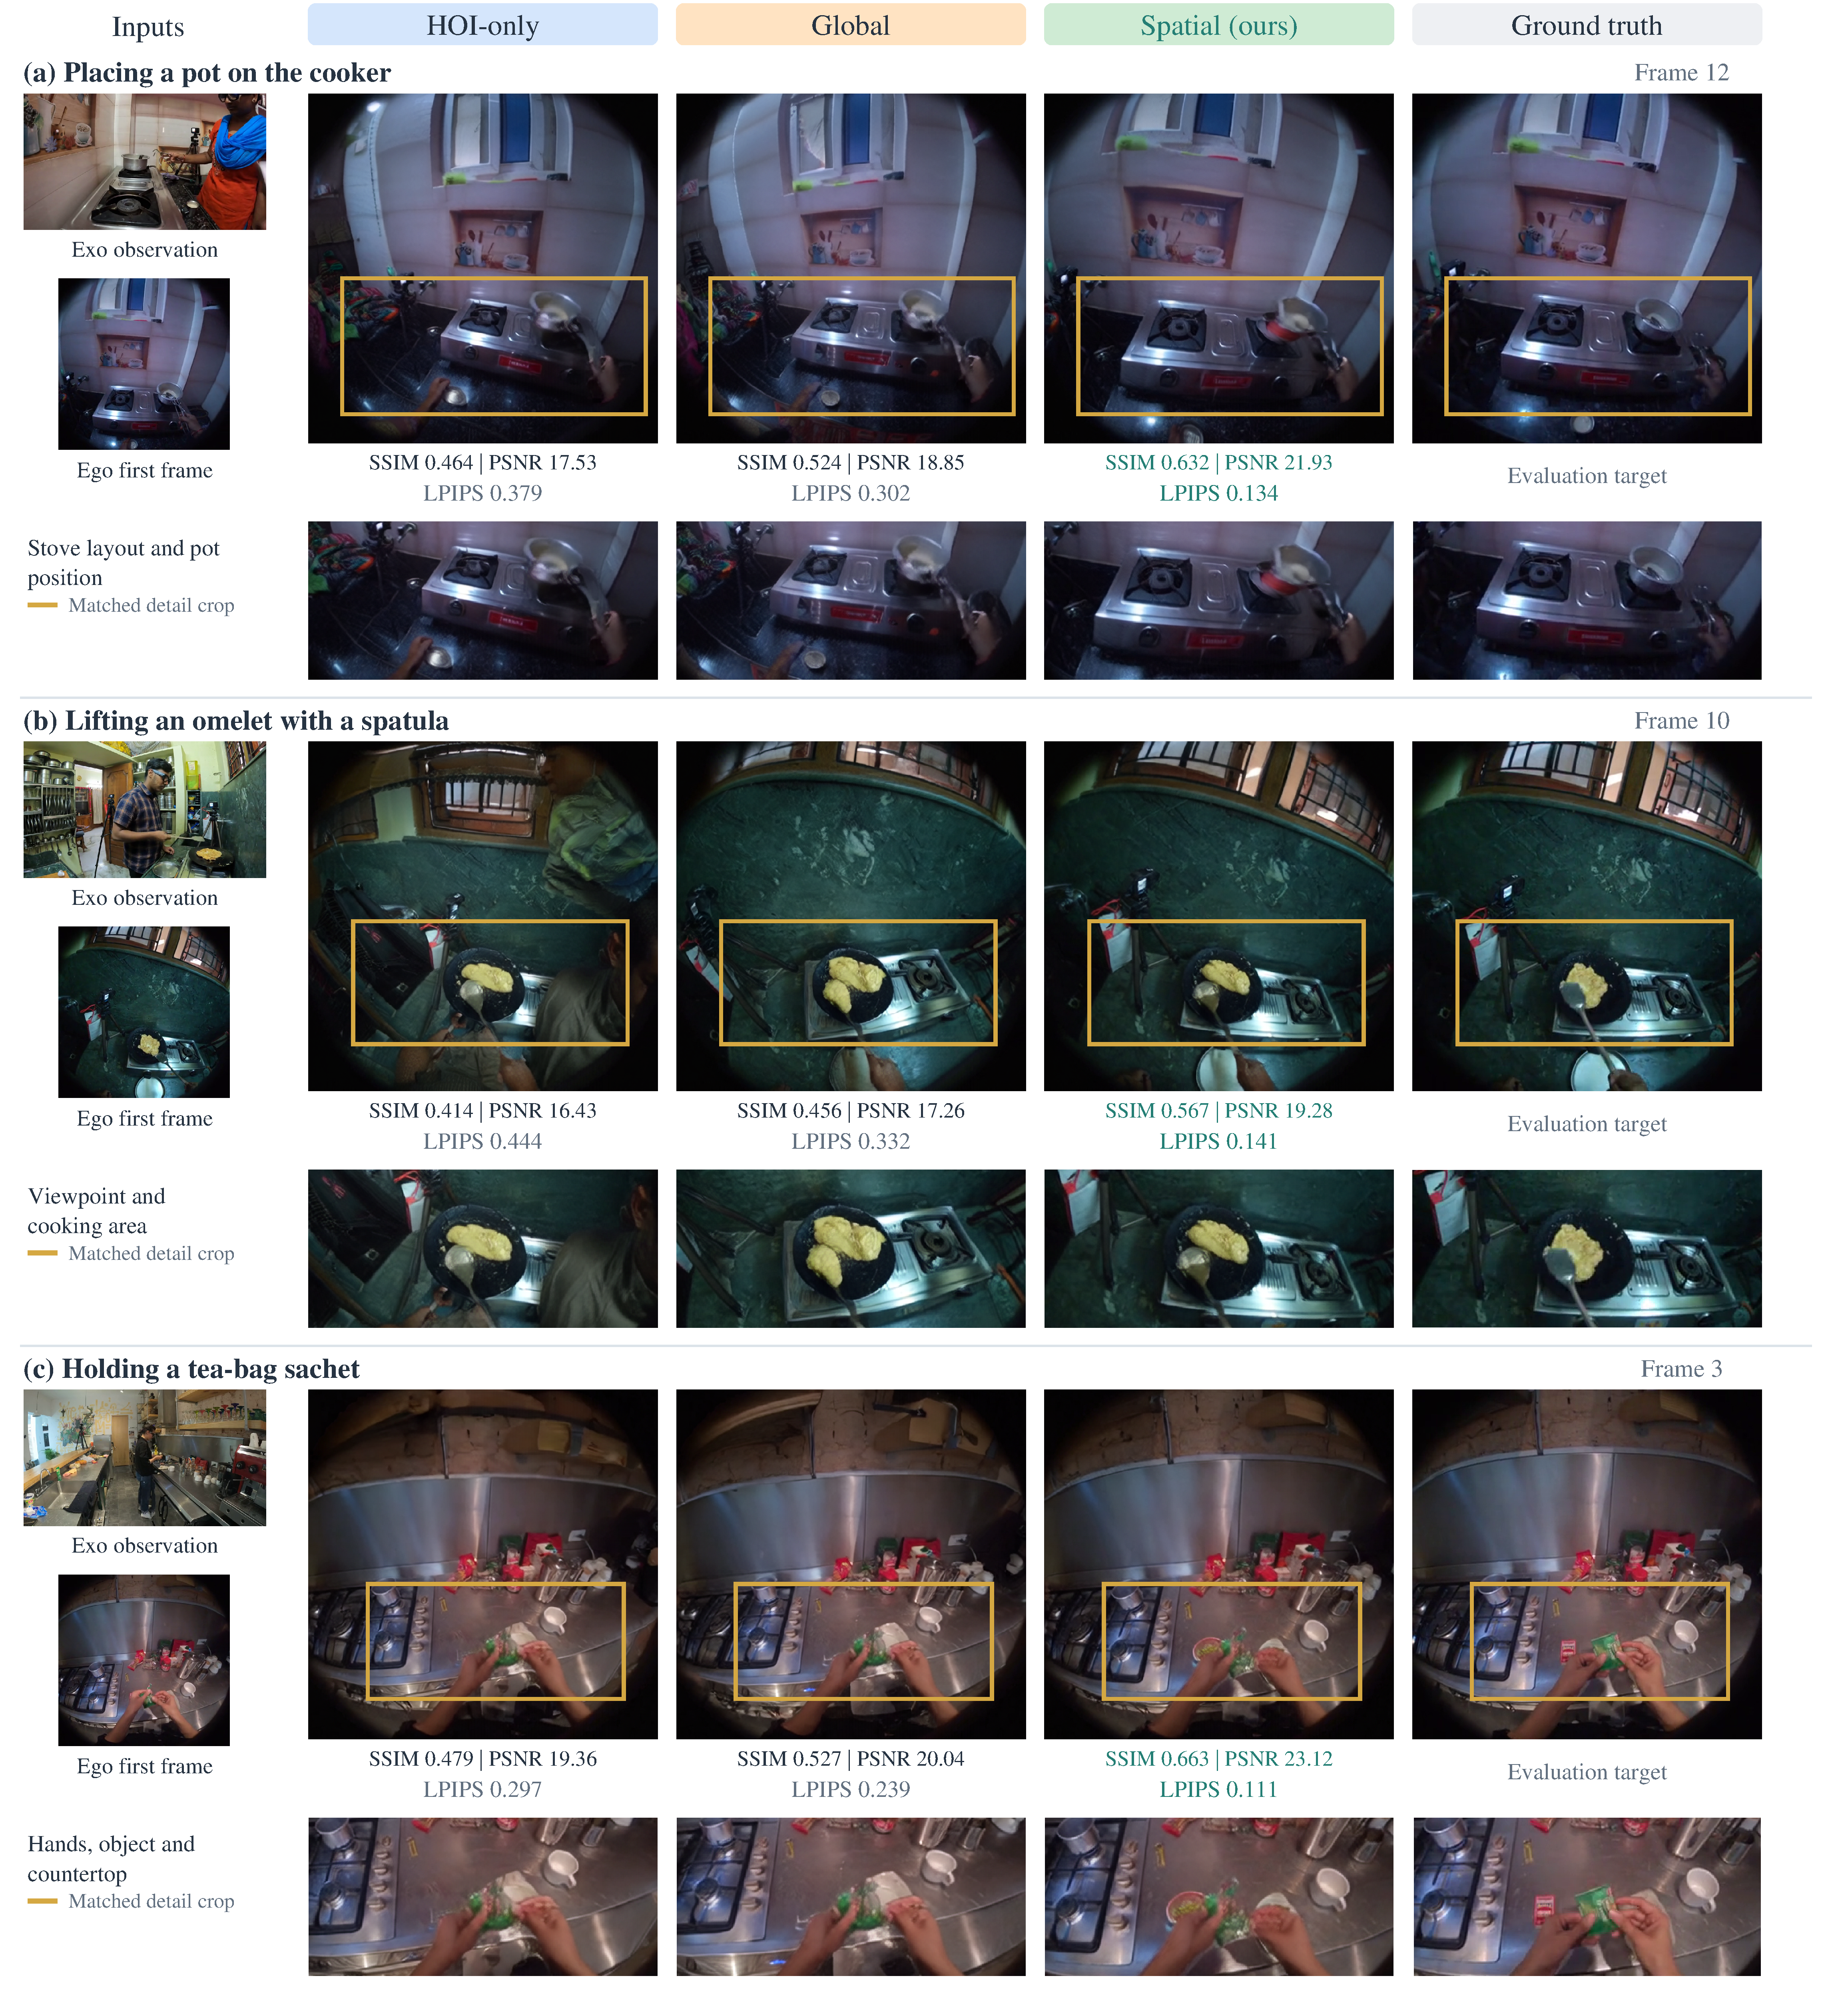
\includegraphics[width=\textwidth]{figs/appendix_cases.pdf}
\caption{Additional qualitative comparisons from the $N{=}1{,}000$ test set:
(a) placing a pot on the cooker (frame 12), (b) lifting an omelet with a spatula
(frame 10), and (c) holding a tea-bag sachet (frame 3); frame indices start at 0.
The left column shows the exo observation and ego first frame. The remaining
columns compare HOI-only, Global, Spatial, and ground truth. Gold boxes mark
the same crop coordinates across methods; enlarged details appear below.
SSIM ($\uparrow$), PSNR ($\uparrow$, dB), and LPIPS ($\downarrow$) are computed
on the full 13-frame clip, rather than the displayed frame or crop.}
\label{fig:appendix-cases}
\end{figure}


\clearpage
\subsection{Per-clip score distributions}
\label{app:score-distributions}
Figure~\ref{fig:metric-distributions} uses every clip in the fixed
$N{=}1{,}000$ manifest. Each per-clip score is computed over its 13 frames.
Spatial's 10th--90th percentile intervals are $[0.566,0.760]$ for SSIM
and $[19.02,25.22]$ dB for PSNR. Both distributions are approximately
symmetric, with sample skewness $0.23$ and $-0.10$, respectively.
These distributions describe score location and spread; split separation
and coverage are established from the manifests and source metadata.

\begin{figure}[ht]
\centering
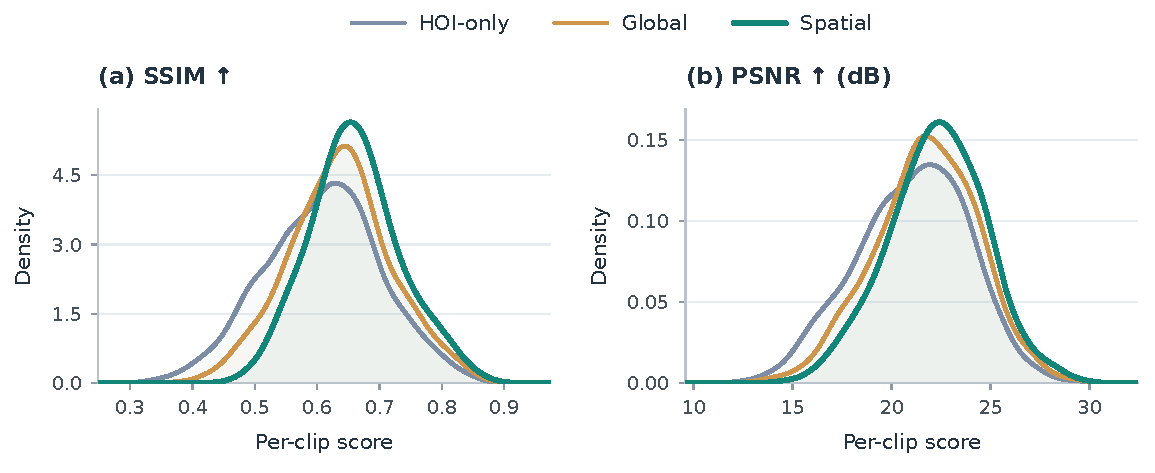
\includegraphics[width=\textwidth]{figs/metric_distributions_ssim_psnr.pdf}
\caption{Per-clip (a) SSIM and (b) PSNR distributions on the fixed
$N{=}1{,}000$ evaluation clips. Curves show Gaussian-kernel density
estimates using all observations. Within each metric, the three methods
share bandwidth $h=s_{\mathrm{pool}}N^{-1/5}$, where
$s_{\mathrm{pool}}$ is the pooled sample standard deviation. Higher scores indicate closer agreement
with the reference videos. The evaluation manifest is the same as in
Table~\ref{tab:phase2-testpool}.}
\label{fig:metric-distributions}
\end{figure}

\end{document}
